\newpage

\section{Оптимальный размер выборки для построения линейных моделей}
Планирование эксперимента требует оценки минимального размера выборки: количества выполненных измерений набора характеристик, необходимых для построения сформулированных условий. Выбор метода оценки размера выборки зависит от решаемой задачи, которая определяет формулировку статистической гипотезы и статистики для ее проверки. В таблице \ref{table1} представлены десять методов оценки размера выборки. Он включает как классический, так и байесовский методы оценки размера выборки.

Классические методы предполагают, что образец соответствует некоторым предварительным условиям, сформулированным ранее. Эти условия сформулированы как статистический критерий (Self et al. 1988, 1992; Shieh 2000; Demidenko 2007). Метод оценки размера выборки, связанный с этим критерием, гарантирует достижение фиксированной статистической мощности $1-\beta$ со степенью ошибки первого рода, не превышающей установленное значение $\alpha$. Такой размер выборки называется достаточным.

\begin{table}
\begin{center}
\caption{Methods}
\label{table1}
\resizebox{\textwidth}{!}{
\begin{tabular}{|p{0.15\textwidth}|p{0.6\textwidth}|p{0.15\textwidth}|}
\hline
	\centering Метод &\centering Описание & Ссылка\\
\hline
	Lagrange multipliers test &
	Правдоподобие выборки имеет следующий вид:
   	$p(y|\textbf{x}, \textbf{w}) = \exp\bigl(y\theta- b(\theta) + c\left(y\right)\bigr).$
	Достаточный размер выборки $m^*$:
	$m^* = \frac{\gamma^*}{\gamma^0}$, где $\gamma^*$ и $\gamma_0$ задаются выражениям \eqref{eq:sb:6} и \eqref{eq:sb:5}.
	&Self et al. 1988\\
\hline
	Likelihood ratio test&
	Правдоподобие выборки имеет следующий вид:
	$p(y|\textbf{x}, \textbf{w}) = \exp\left(\frac{y\theta- b(\theta)}{a(\phi)} + c\left(y, \phi\right)\right).$
	Достаточный размер выборки $m^*$:
	$m^* = \frac{\gamma^*}{\Delta^*},$ где $\gamma^*$ и $\Delta^*$ задаются вывражениями \eqref{eq:sb:11} и \eqref{eq:sb:13}.
	&Shieh 2000\\
\hline
	Wald statistic&
	Правдоподобие выборки имеет следующий вид:
	$p(y|\textbf{x}, \textbf{w}) = \exp\left(\frac{y\theta- b(\theta)}{a(\phi)} + c\left(y, \phi\right)\right).$
	
	Достаточный размер выборки $m^*$:
	
	$m^* = \frac{\gamma^*}{\delta},$ где $\gamma^*$ и $\delta$ задаются выражением \eqref{eq:sb:20}.
	&Shieh 2005\\
\hline
	Cross-validation&
	
	Достаточный размер выборки $m^*$:
	
	$ \forall m \geq m^* RS(m) \geq 1- \varepsilon,$
	где $\varepsilon$ задается экспертно, $RS$ определяется выражением \eqref{eq:hb:5}.
	&Motrenko et al. 2014\\
\hline
	Bootstrap&
	
	Достаточный размер выборки $m^*: \forall m\geq m^* \max_i\left(b^m_i - a^m_i\right) < l$, где $(a^m_i,  b^m_i)$ является квантилью доверительного интервала $i$-й бутсрап подвыборки размера $m$

	&(Qumsiyeh 2013)\\
\hline
	Kullback-Leibler&
	
	Достаточный размер выборки $m^*$:
	
	$\forall \mathfrak{D}_{\mathcal{B}_1}: \left|\mathfrak{D}_{\mathcal{B}_1}\right| \geq m^*    \mathsf{E}_{\mathfrak{D}_{\mathcal{B}_2}}D_\text{KL}\left(p_1, p_2\right) \leq \varepsilon,$
	где $\mathcal{B}_1, \mathcal{B}_2$ удовлетворяет \eqref{eq:bs:8}.
	&Motrenko et al. 2014\\
\hline
	Average posterior variance criterion&
	
	Достаточный размер выборки $m^*$:
	
	$\forall m \geq m^*    \mathsf{E}_{\mathfrak{D}_m}\mathsf{D}\left[\hat{\textbf{w}}|\mathfrak{D}_m\right] \leq \varepsilon,$ где $\varepsilon$  достаточно малое значение.
	&Joseph et al. 1997, 1995\\
\hline
	Average coverage criterion&
	Достаточный размер выборки $m^*$:
	
	$\forall m \geq m^*    \mathsf{E}_{\mathfrak{D}_m}\mathsf{P}\left\{\textbf{w} \in A\left(\mathfrak{D}_m\right)\right\} \geq 1-\alpha$, где $\alpha$ достаточно малое значение.
	&Joseph et al. 1997, 1995\\
\hline
	Average length criterion&
	Достаточный размер выборки $m^*$:
	
	$\forall m \geq m^*    \mathsf{E}_{\mathfrak{D}_m}r_m\leq l,$ 
	where $r_m$ is described in \eqref{eq:bs:5}
	&Joseph et al. 1997, 1995\\
\hline
	Utility maximization&
	Достаточный размер выборки $m^*$:
	
	$m^* = \argmax_{m} \mathsf{E}_{\mathfrak{D}_m}\int_{\textbf{w}}u\left(\mathfrak{D}, \textbf{w}\right)p(\textbf{w}|\mathfrak{D})d\textbf{w},$
	где функция полезности $u\left(\mathfrak{D}, \textbf{w}\right)$ задается выражением \eqref{eq:bs:7}.
	&Lindley 1997\\


\hline
\end{tabular}
}
\end{center}
\end{table}

Однако практическое применение методов оценки размера выборки предполагает, что модель соответствует измеренным данным (Kloek, 1975). Эти модели выбираются в соответствии с постановкой задачи регрессии или классификации. В этой статье представлены обобщенные линейные модели. В статье (Self et al. 1988) описывается метод оценки мощности критерия множителя Лагранжа для коэффициентов обобщенной линейной регрессии, с помощью которого оценивается размер выборки. Недостаток данного метода заключается в том, что, когда альтернативная гипотеза сильно отличается от нулевой гипотезы, оценки максимального правдоподобия для параметров модели и ковариационная матрица, используемые для оценки мощности, не являются асимптотически согласованными в альтернативной гипотезе. Позднее (Self et al. 1992) был предложен подход к оценке мощности и размера выборки, связанной с ней, на основе теста отношения максимального правдоподобия. Этот подход оказался более точным для ряда независимых переменных. Кроме того, в статье (Shieh 2005) был предложен метод оценки мощности для статистики Вальда. В статье (Мотренко и др., 2014) в случае логистической регрессии предлагается использовать метод, использующий кривую ROC-AUC и концепцию сдвига. Классические методы (Self et al. 1988, 1992; Shieh 2000, 2005; Demidenko 2007) имеют ряд ограничений, связанных с практическим применением этих методов. Чтобы оценить размер выборки, необходимо знать дисперсию оценки параметра или, в более общем случае, иметь оценку параметра нецентральности в распределении статистики, используемой, когда альтернативная гипотеза верна. Эти методы не показывают, как получить эти значения. Кроме того, дисперсия оценки и параметр нецентральности не будут получены с определенной дисперсией, влияние которой на результат оценки размера выборки не имеет значения.

Статистические методы позволяют оценить размер выборки на основе предположений о распределении данных и информации о соответствии между наблюдаемыми значениями и предположениями нулевой гипотезы. Когда размер исследуемой выборки является достаточным или чрезмерным, можно использовать методы, основанные на наблюдении изменения определенной характеристики процедуры построения модели при увеличении размера выборки. В частности, наблюдая за соотношением качества прогнозирования с контрольной выборкой и обучающей выборкой (Мотренко и др., 2014), мы будем определять достаточный размер выборки, который соответствует началу переобучения. В статье (Qumsiyeh 2013) для оценки достаточного размера выборки используется метод ресемплирования выборки используя процедуру бутстрап. Превышение текущего размера выборки проверяется на основе анализа доверительных интервалов оцениваемого параметра. Ширина доверительного интервала с разными значениями объема выборки оценивается с помощью метода бутстрапа. Для этого выборки меньшего размера отбираются заданное количество раз и вычисляется доверительный интервал ошибки при оценке параметра модели. Размер выборки считается достаточным, если ширина доверительного интервала не превышает заранее установленного значения.

Перечисленные выше ограничения статистических методов оценки размера выборки подробно рассматриваются в байесовской процедуре (Lindley 1997; Rubin et al. 1998; Wang et al. 2002), где оценка размера выборки определяется на основе максимизации ожидаемого значение некоторой функции качества (Lindley 1997). Функция качества может включать в себя явные функции распределения параметров и штрафы за увеличение размера выборки. Альтернативой подходам (Wang et al. 2002), основанным на функции качества, является выборка размера выборки путем установления ограничений на определенный критерий качества оценки параметров модели. Примеры таких критериев следующие: критерий средней апостериорной дисперсии (AVPC), критерий средней длины (ALC), критерий среднего покрытия (ACC). Для каждого перечисленного критерия оценка размера выборки определяется как минимальное значение размера выборки, для которого ожидаемое значение выбранного критерия не превышает какого-либо фиксированного порога. В статье (Motrenko et al. 2014) предлагается считать размер выборки достаточным, если расстояние Кульбака-Лейблера между распределениями, оцененными на основе подвыборок такого размера, достаточно мало. Такой подход не требует дальнейшего обобщения в случае нескольких переменных. Кроме того, оценка может производиться как при наличии предположений о распределении данных, так и при их отсутствии. Недостаток этого подхода заключается в том, что количественная оценка может быть получена только при чрезмерно большом размере выборки.

\subsection{Постановка задачи определения оптимального размера выборки}

Задана выборка размера $m$:
\[
\label{eq:ps:1}
\begin{aligned}
	\mathfrak{D}_{m} = \{\textbf{x}_i, y_i\}_{i = 1}^{m},
\end{aligned}
\]
где $\textbf{x}_i\in \mathbb{R}^{n}$, $y_i\in \mathbb{Y}$. Вектор признаков $\textbf{x} = [\textbf{u}, \textbf{v}]$ соединяет $\textbf{u}_i\in \mathbb{R}^{k}$ and $ \textbf{v}_i\in \mathbb{R}^{n-k}$.
Выборка $\mathfrak{D}_{m}$ случайным образом делиться на обучающую и тестовую части:
\[
\label{eq:ps:2}
\begin{aligned}
	\mathfrak{D}_{\mathcal{T}_{m}} = \{\textbf{x}_i, \textbf{y}_i\}_{i \in \mathcal{T}_{m}}, \quad \mathfrak{D}_{\mathcal{L}_{m}} = \{\textbf{x}_i, \textbf{y}_i\}_{i \in \mathcal{L}_{m}}, \quad  \mathcal{T}_{m}\sqcup\mathcal{L}_{m} = \{1, ..., m\}.
\end{aligned}
\]
Введем параметрическое семейство функций для аппроксимации неизвестного распределения $p(y|\textbf{x}, \mathfrak{D}_{\mathcal{L}_{m}})$:
\[
\label{eq:ps:3}
\begin{aligned}
	\mathfrak{F} = \left\{f\left(y,\textbf{x}, \textbf{w}\right)|\textbf{w}\in\mathbb{W}, \int_{y\in \mathbb{Y}, \textbf{x}\in\mathbb{R}^{n}}f\left(y, \textbf{x}, \textbf{w}\right)dyd\textbf{x}=1\right\}.
\end{aligned}
\]

Для модели $f$ с вектором параметров $\textbf{w}$ определим функцию правдоподобия и логарифм функции прадоподобия выборки $\mathfrak{D}$:
\[
\label{eq:ps:4}
\begin{aligned}
	L\left(\mathfrak{D}, \textbf{w}\right) = \prod f\left(y,\textbf{x}, \textbf{w}\right),\quad l\left(\mathfrak{D}, \textbf{w}\right) = \sum \log f\left(y,\textbf{x}, \textbf{w}\right),
\end{aligned}
\]
где $f(y,\textbf{x}, \textbf{w})$ является оценкой правдоподобия выборки $\mathfrak{D}_{\mathcal{L}}$ с заданым вектором параметров $\textbf{w}$.
Используйте принцип максимального правдоподобия для оценки параметров $\textbf{w}$
\[
\label{eq:ps:5}
\begin{aligned}
	\hat{\textbf{w}} = \argmax_{\textbf{w}\in\mathbb{W}}L\left(\mathfrak{D}_{\mathcal{L}}, \textbf{w}\right).
\end{aligned}
\]

Информационная матрица Фишера имеет вид:
\[
\label{eq:ps:6}
\begin{aligned}
	\textbf{I}\left(\mathfrak{D}, \textbf{w}\right) = -\nabla\nabla^{\mathsf{T}}l\left(\mathfrak{D}, \textbf{w}\right), \quad  \textbf{V} = \textbf{I}^{-1}\left(\mathfrak{D}, \textbf{m}\right),
\end{aligned}
\]
статистические методы и байесовские методы используют информационную матрицу Фишера для оценки размера выборки.

\subsection{Обзор методов для определения оптимального размера выборки на основе статистических тестов}
Основным преимуществом методов, основанных на статистике, является их способность оценивать достаточный размер выборки при недостаточном наборе выборки. Они позволяют прогнозировать необходимое количество образцов на ранней стадии эксперимента.

Пусть вероятность имеет следующий вид:
\[
\label{eq:sb:1}
\begin{aligned}
	p(y|\textbf{u},\textbf{v},\textbf{w}_{u},\textbf{w}_{v}) = \exp\bigl(y\theta- b(\theta) + c\left(y\right)\bigr),
\end{aligned}
\]
где $\theta$ является параметром распределения, который вычисляются с помощью функции связи $\theta=\theta\bigr(\textbf{u},\textbf{v},\textbf{w}_{u},\textbf{w}_{v}\bigr)$.

Трестируемая гипотеза
\[
\label{eq:sb:2}
\begin{aligned}
	H_0: \textbf{m}_{u} = \textbf{m}^0_{u}, \quad H_1: \textbf{m}_{u} \not= \textbf{m}^0_{u}.
\end{aligned}
\]

Пусть статистики $S_{m,u}\left(\textbf{w}_{u}, \textbf{w}_{v}\right)$ и $S_{m,v}\left(\textbf{w}_{u}, \textbf{w}_{v}\right)$ являются производными логарифма правдоподобия выборки $\mathfrak{D}_{m}$ в точках $\textbf{w}_{u}$ и $\textbf{w}_{v}$.
Рассмотрим $\textbf{s}_{m} = S_{m,u}\left(\textbf{m}^{0}_{u}, \hat{\textbf{w}}^{0}_{v}\right)$, где $\hat{\textbf{w}}^{0}_{v}$ получается из уравнения
\[
\label{eq:sb:3}
\begin{aligned}
	S_{m,v}\left(\textbf{m}^{0}_{u}, \textbf{w}_{v}\right) = 0.
\end{aligned}
\]

Статистика Лагранджа равняется
\[
\label{eq:sb:4}
\begin{aligned}
	LM = \textbf{s}^{\mathsf{T}}_{m}\textbf{Q}_{m}^{-1}\textbf{s}_{m}.
\end{aligned}
\]
где $\textbf{Q}_{m}$ ковариационная матрица вектора $\textbf{s}_{m}$.
	
В случае истинности гипотезы $H_0$ статистика $LM$ асимптотически имеет распределения $\chi^2(k)$.  В работе (Self et al. 1988) показано, что при альтернативной гипотезе $H_1$ статистика  $LM$ асимптотически имеет распределения $\chi^2(k,\gamma)$, где $\gamma$ является параметром не центральности
\[
\label{eq:sb:5}
\begin{aligned}
	\gamma = \bm{\xi}_{m}^{\mathsf{T}}\bm{\Sigma}^{-1}_{m}\bm{\xi}_{m} = m\bm{\xi}^{\mathsf{T}}\bm{\Sigma}^{-1}\bm{\xi}= m\gamma^0,
\end{aligned}
\]
где $\bm{\xi}_{m}$ и $\bm{\Sigma}_{m}$ матрицы математического ожидания и ковариации $\textbf{s}_{m}$. Обозначим $\bm{\xi}_1 = \bm{\xi}$,  $\bm{\Sigma}_1 = \bm{\Sigma}$. 
	
Альтернативный метод получения $\gamma$ включает условия на уровне значимости $\alpha$ и вероятность ошибки II рода $\beta$:
\[
\label{eq:sb:6}
\begin{aligned}
	\gamma^*:\chi^2_{k, 1-\alpha} = \chi^2_{k, \beta}\left(\gamma\right).
\end{aligned}
\]
Используя \eqref{eq:sb:5} и \eqref{eq:sb:6} получаем
\[
\label{eq:sb:7}
\begin{aligned}
	m^* = \frac{\gamma^*}{\gamma^0}.
\end{aligned}
\]
Это достаточный минимальный размер выборки, чтобы различить вектор $\textbf{m}_{u}$ от $\textbf{m}^0_{u}$.

Пусть правдоподобие выборки задается выражением
\[
\label{eq:sb:8}
\begin{aligned}
	p(y|\textbf{u},\textbf{v},\textbf{w}_{u},\textbf{w}_{v}) = \exp\left(\frac{y\theta- b(\theta)}{a(\phi)} + c\left(y, \phi\right)\right),
\end{aligned}
\]
где $\theta$ является параметром распределения, который вычисляются с помощью функции связи $\theta=\theta\bigr(\textbf{u},\textbf{v},\textbf{w}_{u},\textbf{w}_{v}\bigr)$.

Проверяемая гипотеза:
\[
\label{eq:sb:9}
\begin{aligned}
	H_0: \textbf{m}_{u} = \textbf{m}^0_{u}, \quad H_1: \textbf{m}_{u} \not= \textbf{m}^0_{u}.
\end{aligned}
\]
Введем логарифм статистики отношения правдоподобий:
\[
\label{eq:sb:10}
\begin{aligned}
	LR = 2\Big(l\left(\mathfrak{D}, \hat{\textbf{w}}\right) - l\left(\mathfrak{D}, \hat{\textbf{w}}^0\right)\Big),
\end{aligned}
\]
где $\hat{\textbf{w}} = [\hat{\textbf{w}}_{u},\hat{\textbf{w}}_{v}]$ является вектором, который максимизирует правдоподобие \eqref{eq:sb:8}, $\hat{\textbf{w}}^{0} = [\textbf{m}^{0}_{u},\hat{\textbf{w}}^{0}_{v}]$ является вектором, который максимизирует правдоподобие \eqref{eq:sb:8} с фиксируемым подвектором параметров $\textbf{m}^{0}_{u}$.

В случае истинности гипотезы $H_0$ статистика $LR$ асимптотически имеет распределения $\chi^2(k)$.  В работе (Shieh 2000) показано, что при альтернативной гипотезе $H_1$ статистика  $LR$ асимптотически имеет распределения $\chi^2(k,\gamma)$, где $\gamma$ является параметром не центральности
\[
\label{eq:sb:11}
\begin{aligned}
	\gamma = m\Delta^*, \quad \Delta^* = \mathsf{E}\left[2a^{-1}(\phi)\left\{\left(\theta - \theta^*\right)\nabla b(\theta) - b(\theta) + b(\theta^*)\right\}\right], 
\end{aligned}
\]
где параметры $\theta$ и $\theta^*$ рассчитываются используя параметры $\textbf{w} = [\textbf{w}_{u}, \textbf{w}_{v}]$ и $\textbf{w}^* = [\textbf{w}^{0}_{u}, \textbf{w}^{*}_{v}]$. Параметры $\textbf{w}^{*}_{v}$ вычисляются на основе решения уравнения:
\[
\label{eq:sb:12}
\begin{aligned}
	\lim_{m\to\infty}m^{-1}\mathsf{E}\left(\frac{\partial l\left(\mathfrak{D}, \left[\textbf{m}^{0}_{u}, \textbf{w}_{v}\right]\right)}{\partial \textbf{w}_{v}}\right) = 0.
\end{aligned}
\]
	
Тогда с учетом $\alpha$ и $\beta$ достаточный размер выборки  $m^*$ вычисляется следующим образом:
\[
\label{eq:sb:13}
\begin{aligned}
	m^* = \frac{\gamma^*}{\Delta^*}, \quad \gamma^*:\chi^2_{k, 1-\alpha} = \chi^2_{k, \beta}\left(\gamma\right), 
\end{aligned}
\]
где $\chi^2_{k, 1-\alpha}$, $\chi^2_{k, \beta}\left(\gamma^*\right)$ квантили распределений $\chi^{2}_k$ and $\chi^2_{k}\left(\gamma^*\right)$.
	
Пусть правдоподобие выборки задается следующим образом:
\[
\label{eq:sb:14}
\begin{aligned}
	p(y|\textbf{u},\textbf{v},\textbf{w}_{u},\textbf{w}_{v}) = \exp\left(\frac{y\theta- b(\theta)}{a(\phi)} + c\left(y, \phi\right)\right),
\end{aligned}
\]
где $\theta$ является параметром распределения, который вычисляются с помощью функции связи $\theta=\theta\bigr(\textbf{u},\textbf{v},\textbf{w}_{u},\textbf{w}_{v}\bigr)$.

Тестируемая гипотеза:
\[
\label{eq:sb:15}
\begin{aligned}
	H_0: \textbf{m}_{u} = \textbf{m}_{u}^{0}, \quad H_1: \textbf{m}_{u} \not=\textbf{m}_{u}^{0}.
\end{aligned}
\]
Тест Вальда для гипотезы:
\[
\label{eq:sb:16}
\begin{aligned}
	W = \left(\hat{\textbf{w}}_{u} - \textbf{m}_{u}^{0}\right)^{\mathsf{T}}\hat{\textbf{V}}_{u}^{-1}\left(\hat{\textbf{w}}_{u} - \textbf{m}_{u}^{0}\right),
\end{aligned}
\]
где $\hat{\textbf{w}} = [\hat{\textbf{w}}_{u},\hat{\textbf{w}}_{v}]$ вектор параметров, который максимизирует правдоподобие выборки \eqref{eq:sb:14}, где матрица $\hat{\textbf{V}}_u$ задается в выражении \eqref{eq:ps:6}.

В случае истинности гипотезы $H_0$ статистика Вальда $W$ асимптотически имеет распределение$\chi^2$. В работе (Shieh 2005) показано, что в случае истинности альтернативной гипотезы $H_1$ статистика Вальда $W$ асимптотически имеет распределение $\chi^2(k,\gamma)$ с параметром не центральности $\gamma$:
\[
\label{eq:sb:17}
\begin{aligned}
	\gamma = m\delta, \quad \delta = \left(\hat{\textbf{w}}_{u} - \textbf{m}_{u}^{0}\right)^{\mathsf{T}}\bm{\Sigma}^{-1}_u\left(\hat{\textbf{w}}_{u} - \textbf{m}_{u}^{0}\right), \quad \bm{\Sigma}_u = m\hat{\textbf{V}}_u.
\end{aligned}
\]

Использую заданный уровень значимости $\alpha$ и заданную ошибку второго рода $\beta$ определим оптимальный размер выборки:
\[
\label{eq:sb:18}
\begin{aligned}
	m^* = \frac{\gamma^*}{\delta}, \quad \gamma^*:\chi^2_{k, 1-\alpha^{*}} = \chi^2_{k, \beta}\left(\gamma\right),
\end{aligned}
\]
где $\chi^2_{k, 1-\alpha^*}$, $\chi^2_{k, \beta}\left(\gamma^*\right)$ квантили распределения, а параметр $\alpha^*$ это поправка на уровни значимости:
\[
\label{eq:sb:19}
\begin{aligned}
	\alpha^* = P\left(\bm{\xi}^{\mathsf{T}}\bm{\Sigma}^{*-1} \bm{\xi} > \chi^2_{k,1 - \alpha}\right), \quad \Sigma^* = \textbf{I}^{-1}\left(\mathfrak{D}, \textbf{w}^*\right),
\end{aligned}
\]
где $\textbf{w}^{*} = \left[\textbf{m}_{u}^{0}, \textbf{w}^{*}_v\right]$ является решением уравнения:
\[
\label{eq:sb:20}
\begin{aligned}
	\lim_{m\to\infty}m^{-1}\mathsf{E}\left(\frac{\partial l\left(\mathfrak{D}, \left[ \textbf{m}_{u}^{0}, \textbf{w}_{v}\right]\right)}{\partial \textbf{w}_{v}}\right) = 0.
\end{aligned}
\]

\subsection{Эвристические методы определения достаточного размера выборки}
В методе, основанном на эвристике, используются популярные статистические эвристики, такие как бутстрап, перекрестная проверка и задание функции полезности .
Введем набор индексов $\mathcal {A} $ для параметров логистической регрессии $\textbf {w} $. Тестируемая гипотеза:
\[
\label{eq:hb:1}
\begin{aligned}
	H_0: j \not\in\mathcal{A} \left(\text{w}_{j} = 0\right), \quad H_1: j \in \mathcal{A}^* \left(\text{w}_{j} \not= 0\right),
\end{aligned}
\]
где $\text{w}_{j}$ является $j$-м элементом вектора $\textbf{w}$.
Установим параметр отступа $ c_0 $ для задачи логистической регрессии:
\[
\label{eq:hb:2}
\begin{aligned}
	H_0: 1-c_0 = p_0, \quad H_1: 1-c_0 = p_1,
\end{aligned}
\]
где $c_0$ оптимальное решение, когда исключен $j$-й элемент вектора.
Используя статистику
\[
\label{eq:hb:3}
\begin{aligned}
	Z = \frac{\hat{p}-p_0}{\sqrt{p_0(1-p_0)}}\sqrt{m}, \quad \hat{p} = \frac{1}{m}\sum_{i=1}^{m}y_i.
\end{aligned}
\]
В случае истинности нулевой гипотезы $H_0$ статистика $Z$ асимптотически имеет распределение $\mathcal{N}\left(0, 1\right)$. В случае истинности альтернативной гипотезы $H_1$ статистика $Z$  асимптотически имеет распределение $ \mathcal{N}\left(p_1-p_0, \sqrt{\frac{p_1(1-p_1)}{p_0(1-p_0)}}\right)$.
      
Достаточный объем выборки задается следующим образом:
\[
\label{eq:hb:4}
\begin{aligned}
	m^* = \frac{p_0(1-p_0)\left(Z_{1-\alpha/2} + Z_{1-\beta}\sqrt{\frac{p_1(1-p_1)}{p_0(1-p_0)}}\right)^2}{(p_1-p_0)^2},
\end{aligned}
\]
где $Z_{1-\alpha/2}$ и $Z_{1-\beta}$ являются квантилями распределения $\mathcal{N}\left(0, 1\right)$.
    
Мы не будем рассматривать этот метод далее, поскольку его можно использовать только для задачи логистической регрессии.
    
Определите критерий переобучения как
\[
\label{eq:hb:5}
\begin{aligned}
	RS(m) = \ln\frac{L(\mathfrak{D}_{\mathcal{L}(m)}, \hat{\textbf{w}})}{L(\mathfrak{D}_{\mathcal{T}(m)}, \hat{\textbf{w}})}, \quad \frac{|\mathcal{T}(m)|}{|\mathcal{L}(m)|} = \text{const} \leq 0.5.
\end{aligned}
\]
Заметим, что
\[
\label{eq:hb:6}
\begin{aligned}
	\lim_{m\to \infty}RS(m) \to 0.
\end{aligned}
\]

Достаточный размер выборки $m^*$ определяется согласно условию:
\[
\label{eq:hb:7}
\begin{aligned}
	m^*: \forall m \geq m^* \mathsf{E}_{\mathfrak{D}_{m}}RS(m) \leq \varepsilon,
\end{aligned}
\]
где $\varepsilon$ некоторый параметр задан экспертно.

Этот метод предполагает, что длины доверительных интервалов квантиля не превышают некоторого фиксированного значения $l$. Для некоторого размера выборки $m$ вычисляются квантильные доверительные интервалы $\left (a^m_1, b^m_1\right), \left(a^m_2, b^m_2 \right), ..., \left(a^m_n, b^m_n \right)$ с уровнем значимости $\alpha$ с использованием начальной загрузки для каждого параметра модели. Достаточный размер выборки задается следующим образом:
\[
\label{eq:hb:8}
\begin{aligned}
	m^*: \forall m\geq m^* \max_i\left(b^m_i - a^m_i\right) < l.
\end{aligned}
\]
    
Обратите внимание, что этот метод является покоординатным. Следовательно, для повышения точности прогноза требуется значительное увеличение размера выборки.
    
\subsection{Байесовский подход к определению оптимального размера выборки}
Байесовские методы оценки размера выборки основаны на ограничении некоторых характеристик модели. Для анализа эффективности определяется функция размера выборки. Увеличение этой функции интерпретируется как снижение эффективности модели. Размер выборки $m^*$ выбирается таким, чтобы исследуемая функция была меньше некоторого порогового значения $\varepsilon$.

\paragraph{Average posterior variance criterion.}
Размер выборки $m^*$ определяется условием:
\[
\label{eq:bs:1}
\begin{aligned}
	\forall m \geq m^*    \mathsf{E}_{\mathfrak{D}_m}\mathsf{D}\left[\hat{\textbf{w}}|\mathfrak{D}_m\right] \leq l.
\end{aligned}
\]
где $l$ некоторый заданный экспертно параметр, который количественно определяет неопределенность оценки параметра.

\paragraph{Average coverage criterion.}
Обозначим через $A\left(\mathfrak{D}\right) \subset \mathbb{R}^n$ некоторый набор параметров модели $\textbf{w}$:
\[
\label{eq:bs:2}
\begin{aligned}
	A\left(\mathfrak{D}\right) = \left\{\textbf{w}:||\textbf{w} - \hat{\textbf{w}}||\leq l\right\},
\end{aligned}
\]
где $l$ --- некоторый фиксированный радиус шара.
Размер выборки $m^*$ определяется критерием среднего покрытия:
\[
\label{eq:bs:3}
\begin{aligned}
	\forall m \geq m^*    \mathsf{E}_{\mathfrak{D}_m}\mathsf{P}\left\{\textbf{w} \in A\left(\mathfrak{D}_m\right)\right\} \geq 1-\alpha,
\end{aligned}
\]
где $\alpha$ некоторый параметр заданный экспертно.
	
\paragraph{Average length criterion.}
Определим функцию $A\left(\mathfrak{D}\right)$ следующим образом:
\[
\label{eq:bs:4}
\begin{aligned}
	\mathsf{P}\left(A\left(\mathfrak{D}\right)\right) =  1- \alpha.
\end{aligned}
\]
Оценки критерия средней длины $m^*$ as in \eqref{eq:bs:3}:
	
\[
\label{eq:bs:5}
\begin{aligned}
	\forall m \geq m^*    \mathsf{E}_{\mathfrak{D}_m}r_m\leq l,
\end{aligned}
\]
где $r_m$ является радиусом шара $A\left(\mathfrak{D}_{m}\right)$.

Методы следующего класса максимизируют ожидание некоторой функции полезности $u\left(\mathfrak{D}, \textbf{w}\right)$ по размеру выборки:
\[
\label{eq:bs:6}
\begin{aligned}
	m^* = \argmax_{m} \mathsf{E}_{\mathfrak{D}_m}\int_{\textbf{w}}u\left(\mathfrak{D}_m, \textbf{w}\right)p(\textbf{w}|\mathfrak{D}_m)d\textbf{w},
\end{aligned}
\]
где функция полезности $u\left(\mathfrak{D}, \textbf{w}\right)$ задается в виде:

\[
\label{eq:bs:7}
\begin{aligned}
	u\left(\mathfrak{D}_m, \textbf{w}\right) = l\left(\mathfrak{D}_m, \textbf{w}\right) - cm,
\end{aligned}
\]
 где $c$ функция штрафов для каждого элемента в наборе выборки.
	 
Будем говорить, что индексы $\mathcal{B}_1,\mathcal{B}_2 \subset \{1,...,m\}$ по соседству, если
\[
\label{eq:bs:8}
\begin{aligned}
	\left|\mathcal{B}_1 \Delta \mathcal{B}_2\right| = 1.
\end{aligned}
\]
Таким образом, $\mathcal{B}_2 $ можно преобразовать в $\mathcal{B}_1$ путем удаления, замены или добавления одного элемента. В работе (Motrenko et al. 2014) показано, что если размер набора выборок $\mathfrak {D}_{\mathcal {B}_1}$ достаточно велик, чем параметры модели $\hat{\textbf {w}}_1$, оптимизированные с помощью $\mathfrak{D}_{\mathcal{B}_1}$, должны находиться в окрестности параметров модели $\hat{\textbf{w}}_2 $, которые оптимизированы с помощью $\mathfrak{D}_{\mathcal {B}_2}$.
	 
Используйте дивергенцию Кульбака-Лейблера в качестве функции близости между распределениями параметров модели, оптимизированных с помощью $\mathfrak{D}_{\mathcal{B}_1}$ и $\mathfrak{D}_{\mathcal{B}_2}$:
\[
\label{eq:bs:9}
\begin{aligned}
	D_\text{KL}\left(p_1, p_2\right) = \int_{\textbf{w}\in\mathbb{W}}p_1(\textbf{w})\log\frac{p_1(\textbf{w})}{p_2(\textbf{w})}d\textbf{w},
\end{aligned}
\]
где $p_1$ and $p_2$ апостериорные вероятности вектора параметров $\textbf{w}$ рассчитаные на подвыборках $\mathfrak{D}_{\mathcal{B}_1}$ и $\mathfrak{D}_{\mathcal{B}_2}$ соответсвенно. Также предполагается, что $\mathfrak{D}_{\mathcal{B}_1}$ и $\mathfrak{D}_{\mathcal{B}_2}$ находятся по соседству.
Достаточный размер выборки $m^*$ оценивается следующим образом:
\[
\label{eq:bs:10}
\begin{aligned}
	\forall \mathfrak{D}_{\mathcal{B}_1}: \left|\mathfrak{D}_{\mathcal{B}_1}\right| \geq m^*    \mathsf{E}_{\mathfrak{D}_{\mathcal{B}_2}}D_{KL}\left(p_1, p_2\right) \leq \varepsilon.
\end{aligned}
\]

	  
\subsection{Вычислительный эксперимент по анализу разных подходов к определению оптимального размера выборки}
\begin{table}[!htp]
\centering
\caption{Описание выборок для эксперимента}
\label{table20}
\resizebox{\textwidth}{!}{
\begin{tabular}{|l|l|c|c|}
\hline
	\centering Выборка & Задача & Число признаков & Размер выборки\\ \hline
	\hline 	Boston Housing 	&regression		&14 & 506\\
	\hline	Diabets  				& regression		&20  & 576\\
	\hline	Forest Fires 			& regression		& 13 & 517\\
  	\hline	Servo 					& regression 	& 4   & 167\\
	\hline	NBA				 		& classification	& 12 & 2235\\
\hline
\end{tabular}
}
\end{table} 

Перечисленные выше методы оценки размера выборки реализованы в пакете Python. Этот пакет можно использовать как для прогнозирования достаточного размера выборки на ранней стадии эксперимента, так и для ретроспективного анализа достаточности набора выборки. Этот пакет также включает некоторые вспомогательные функции для исследования размера выборки и визуализации результатов, как показано на рисунках. Исходный код для службы оценки размера выборки доступен по адресу \mbox{\url{https://github.com/andriygav/SampleSizeLib}}. Код эксперимента и наборы данных, использованные в статье, доступны по адресу \mbox{\url{https://github.com/ttgadaev/SampleSizeEstimation}}.

Этот эксперимент был проведен для анализа свойств методов оценки размера выборки. Эксперимент состоит из трех частей. Во время первой части получаются оценки размера для всех наборов выборок при фиксированных идентичных параметрах методов. Во второй части исследуется зависимость достаточного размера выборки от имеющегося размера выборки. В третьей части исследуется поведение методов в зависимости от изменения параметров методов. В качестве данных использовались пять наборов образцов, описанных в таблице \ref{table20}. Девять методов в строках таблицы \ref{table2} показывают оценки размера выборки для соответствующих наборов данных.
 
\begin{table}[!hbp]
\centering
\caption{Эксперимент по оценке размера выборки для различных наборов выборок}
\label{table2}
\resizebox{\textwidth}{!}{
\begin{tabular}{|l|c|c|c|c|c|}
\hline
Методы и наборы данных                        & Boston Housing & Diabetes & Forest Fires & Servo & NBA \\ \hline\hline
Lagrange Multipliers Test & 18             & 25       & 44          & 38    & 218 \\ \hline
Likelihood Ratio Test     & 17             & 25       & 43          & 18    & 110 \\ \hline
Wald Test                 & 66             & 51       & 46          & 76    & 200 \\ \hline
Cross Validation          & 178            & 441      & 172         & 120   & --   \\ \hline
Bootstrap                 & 113            & 117      & 86          & 60    & 405 \\ \hline
APVC                      & 98             & 167      & 351         & 20    & --   \\ \hline
ACC                       & 228            & 441      & 346         & 65    & --   \\ \hline
ALC                       & 98             & 267      & 516         & 25    & --   \\ \hline
Utility Function          & 148            & 172      & 206         & 105   & 925 \\ \hline
\end{tabular}
}
\end{table}

Эта часть вычислительного эксперимента показывает, как разные методы работают с разными наборами данных. В эксперименте используются следующие наборы данных: Boston Housing (Harrison et al. 1978), Diabetes, Forest Fires, Servo (Quinlan 1992), NBA.
Результат представлен в таблице \ref{table2}. Символ `` - '' в таблице означает, что данных для прогноза недостаточно.

Each method was provided with the whole sample at the start was performed. The parameters of each method for all samples are registered and described in the Table \ref{table3}. Since the Lagrange, Likelihood Ration and Wald tests are asymptotic equivalent the parameters of these methods were set identically. The parameters of the Average Coverage and Average Length methods were set identically as well.

Параметры каждого метода для всех выборок описаны в таблице \ref{table3}. Поскольку критерии Лагранжа, отношения правдоподобия и Вальда асимптотически эквивалентны, параметры этих методов задавались одинаково. Параметры методов <<Average Coverage>> и <<Average Length>> также были заданы идентично.

\begin{table}[h!]
\begin{center}
\caption{Перечень параметров для разных методов оценки объема выборки}
\label{table3}
\resizebox{\textwidth}{!}{
\begin{tabular}{|l|l|c|c|c|c|c|c|}
\hline 
Method& GLM parameters& $l$& $\varepsilon$& $\alpha$& $\beta$\\ \hline
\hline	
Lagrange	Multipliers Test	& $\textbf{w}_{u}^0$ & -- & 0.2& 0.05& 0.2\\
\hline	
Likelihood Ratio Test			& $\textbf{w}_{u}^0$ & -- & 0.2& 0.05& 0.2\\
\hline	
Wald	Test								& $\textbf{w}_{u}^0$ & -- & 0.2& 0.05& 0.2\\
\hline	
Cross Validation 					& -- & -- 	& 0.05& -- & --\\
\hline	
Bootstrap 								& -- & 0.5	& -- & 0.05& --\\
\hline	
APVC 									& -- & 0.5	& -- & -- & --\\
\hline	
ACC 									& -- & 0.25	& -- & 0.05& --\\
\hline	
ALC 										& -- & 0.5	& -- & 0.05& --\\
\hline	
Utility function 						& -- & -- 	& 0.005& -- & --\\
\hline
\end{tabular}
}
\end{center}
\end{table}

The computational experiment was conducted to analyse the described methods. The sample set is the Boston Housing Dataset. Having a full sample set, fix some sample size $m$ and generate series of bootstrap subsamples of size $m$ from the initial sample set. For different values of $m$ compute $m^*$, average them and calculate standard deviation. 

Вычислительный эксперимент проводился для анализа описанных методов. Имея полный набор выборок, фиксируется некоторый размер выборки $m$ и методом бутсрап генерируется серия подвыборок размером $m$. Для разных значений $m$ вычисляется $m^*$.
    
\begin{figure}[h!t]\center
    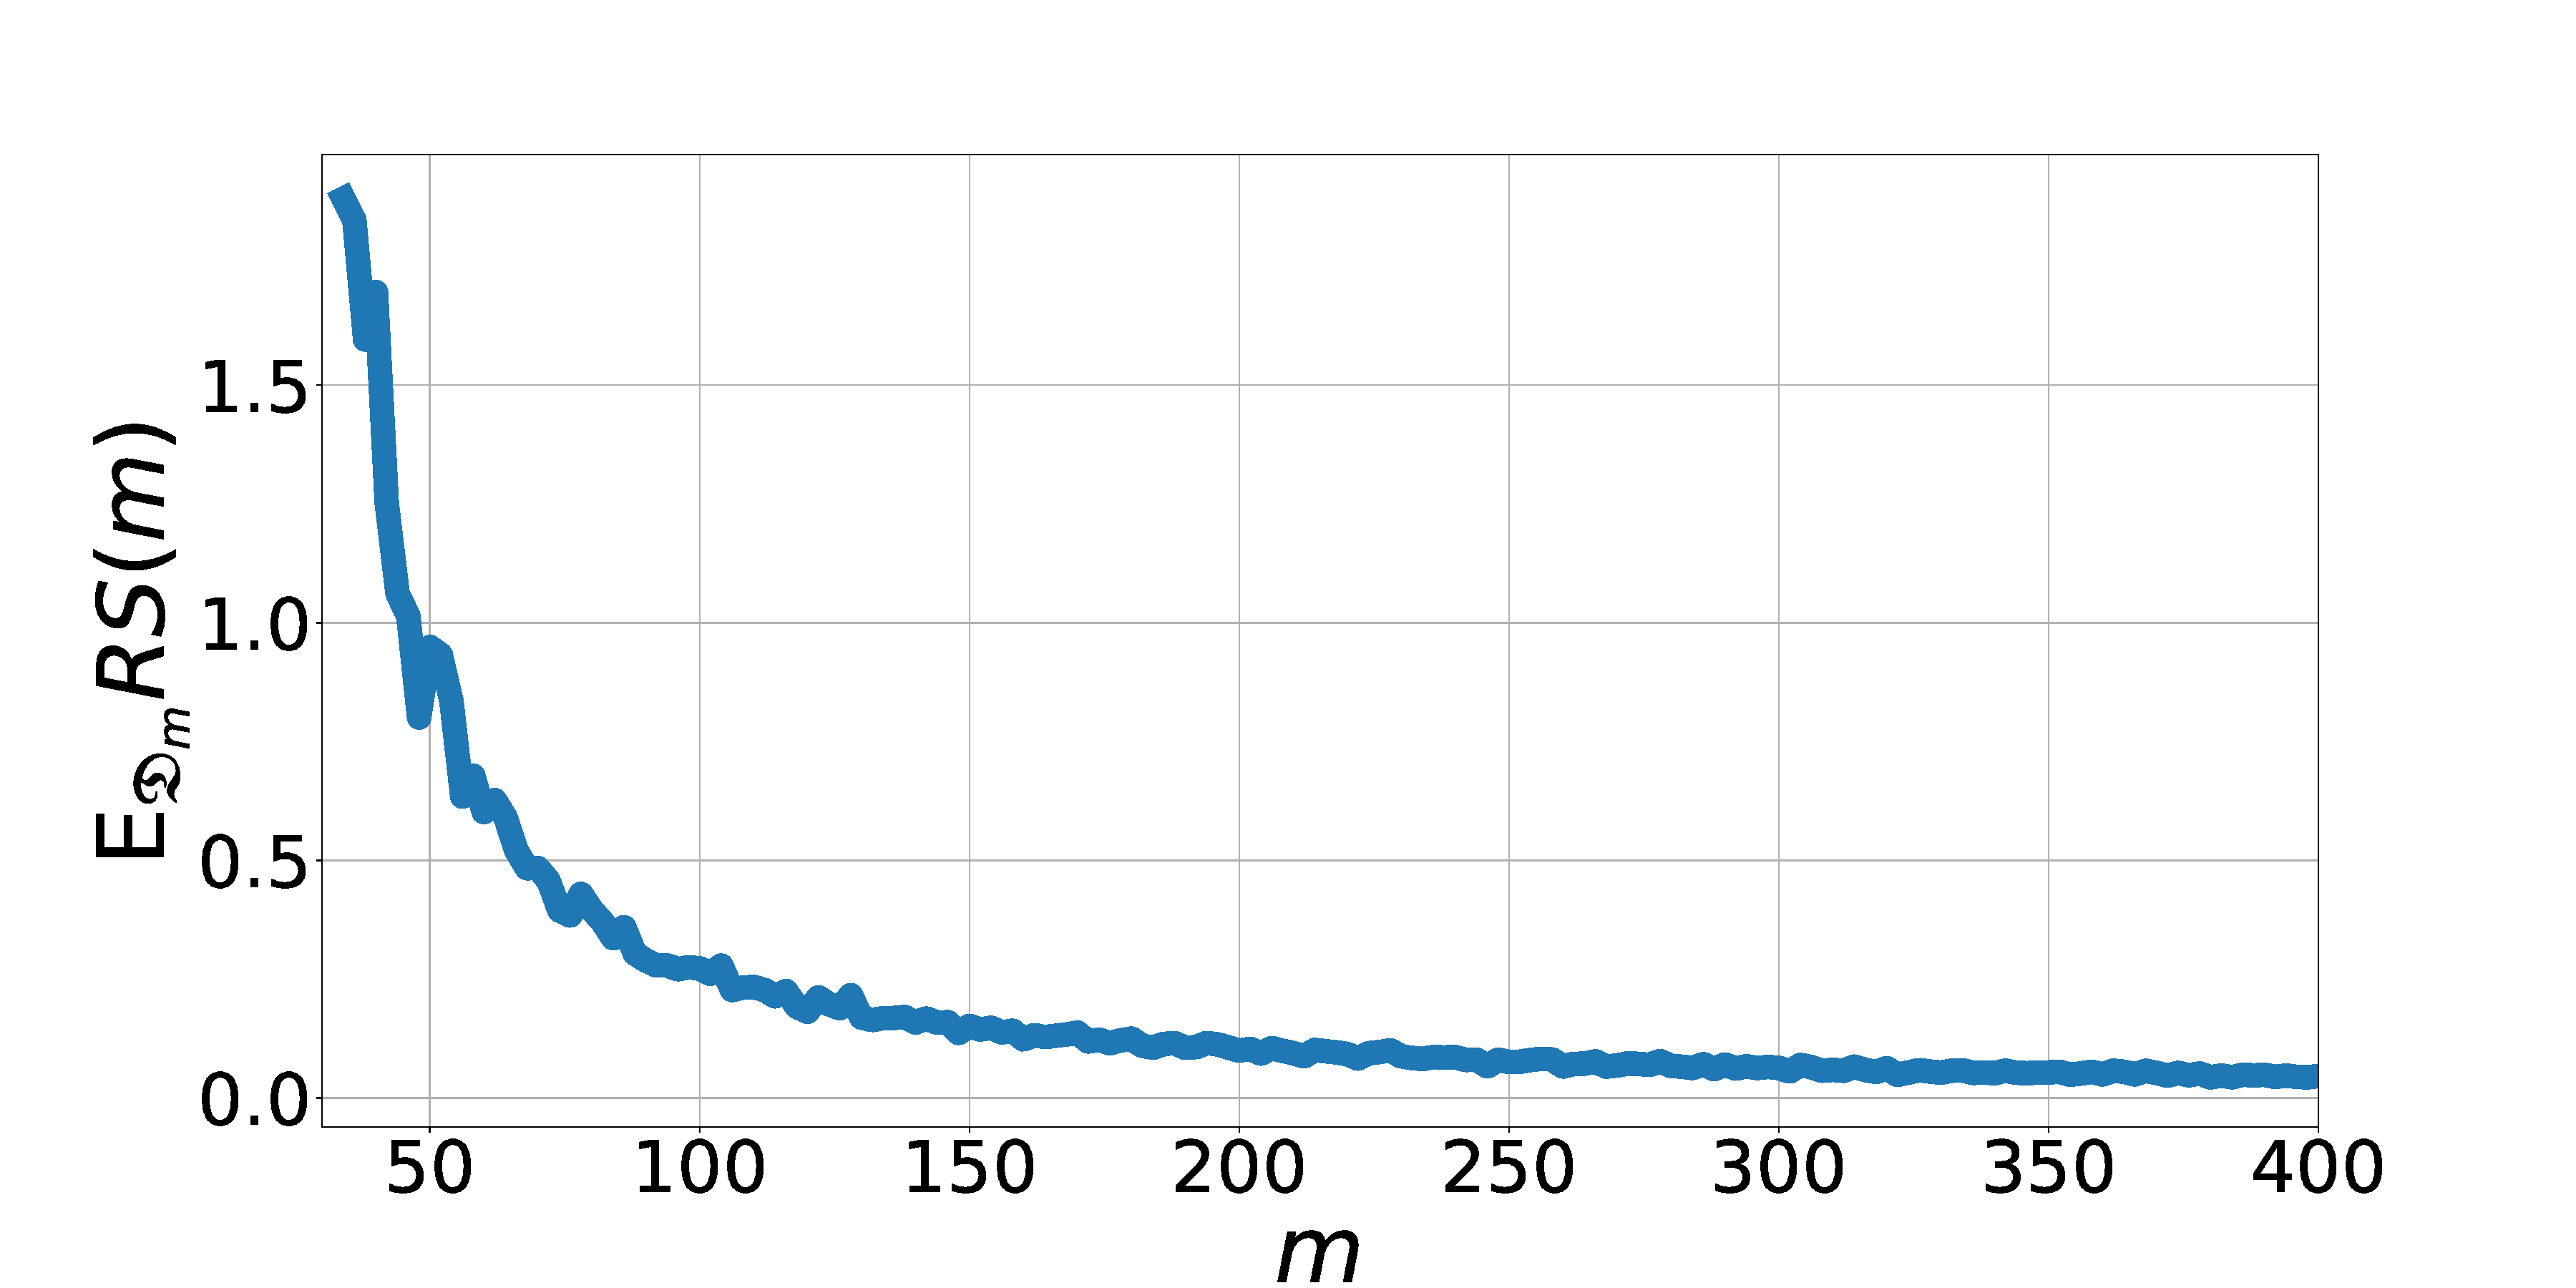
\includegraphics[width=0.49\textwidth]{results/samplesize/cross.pdf}
    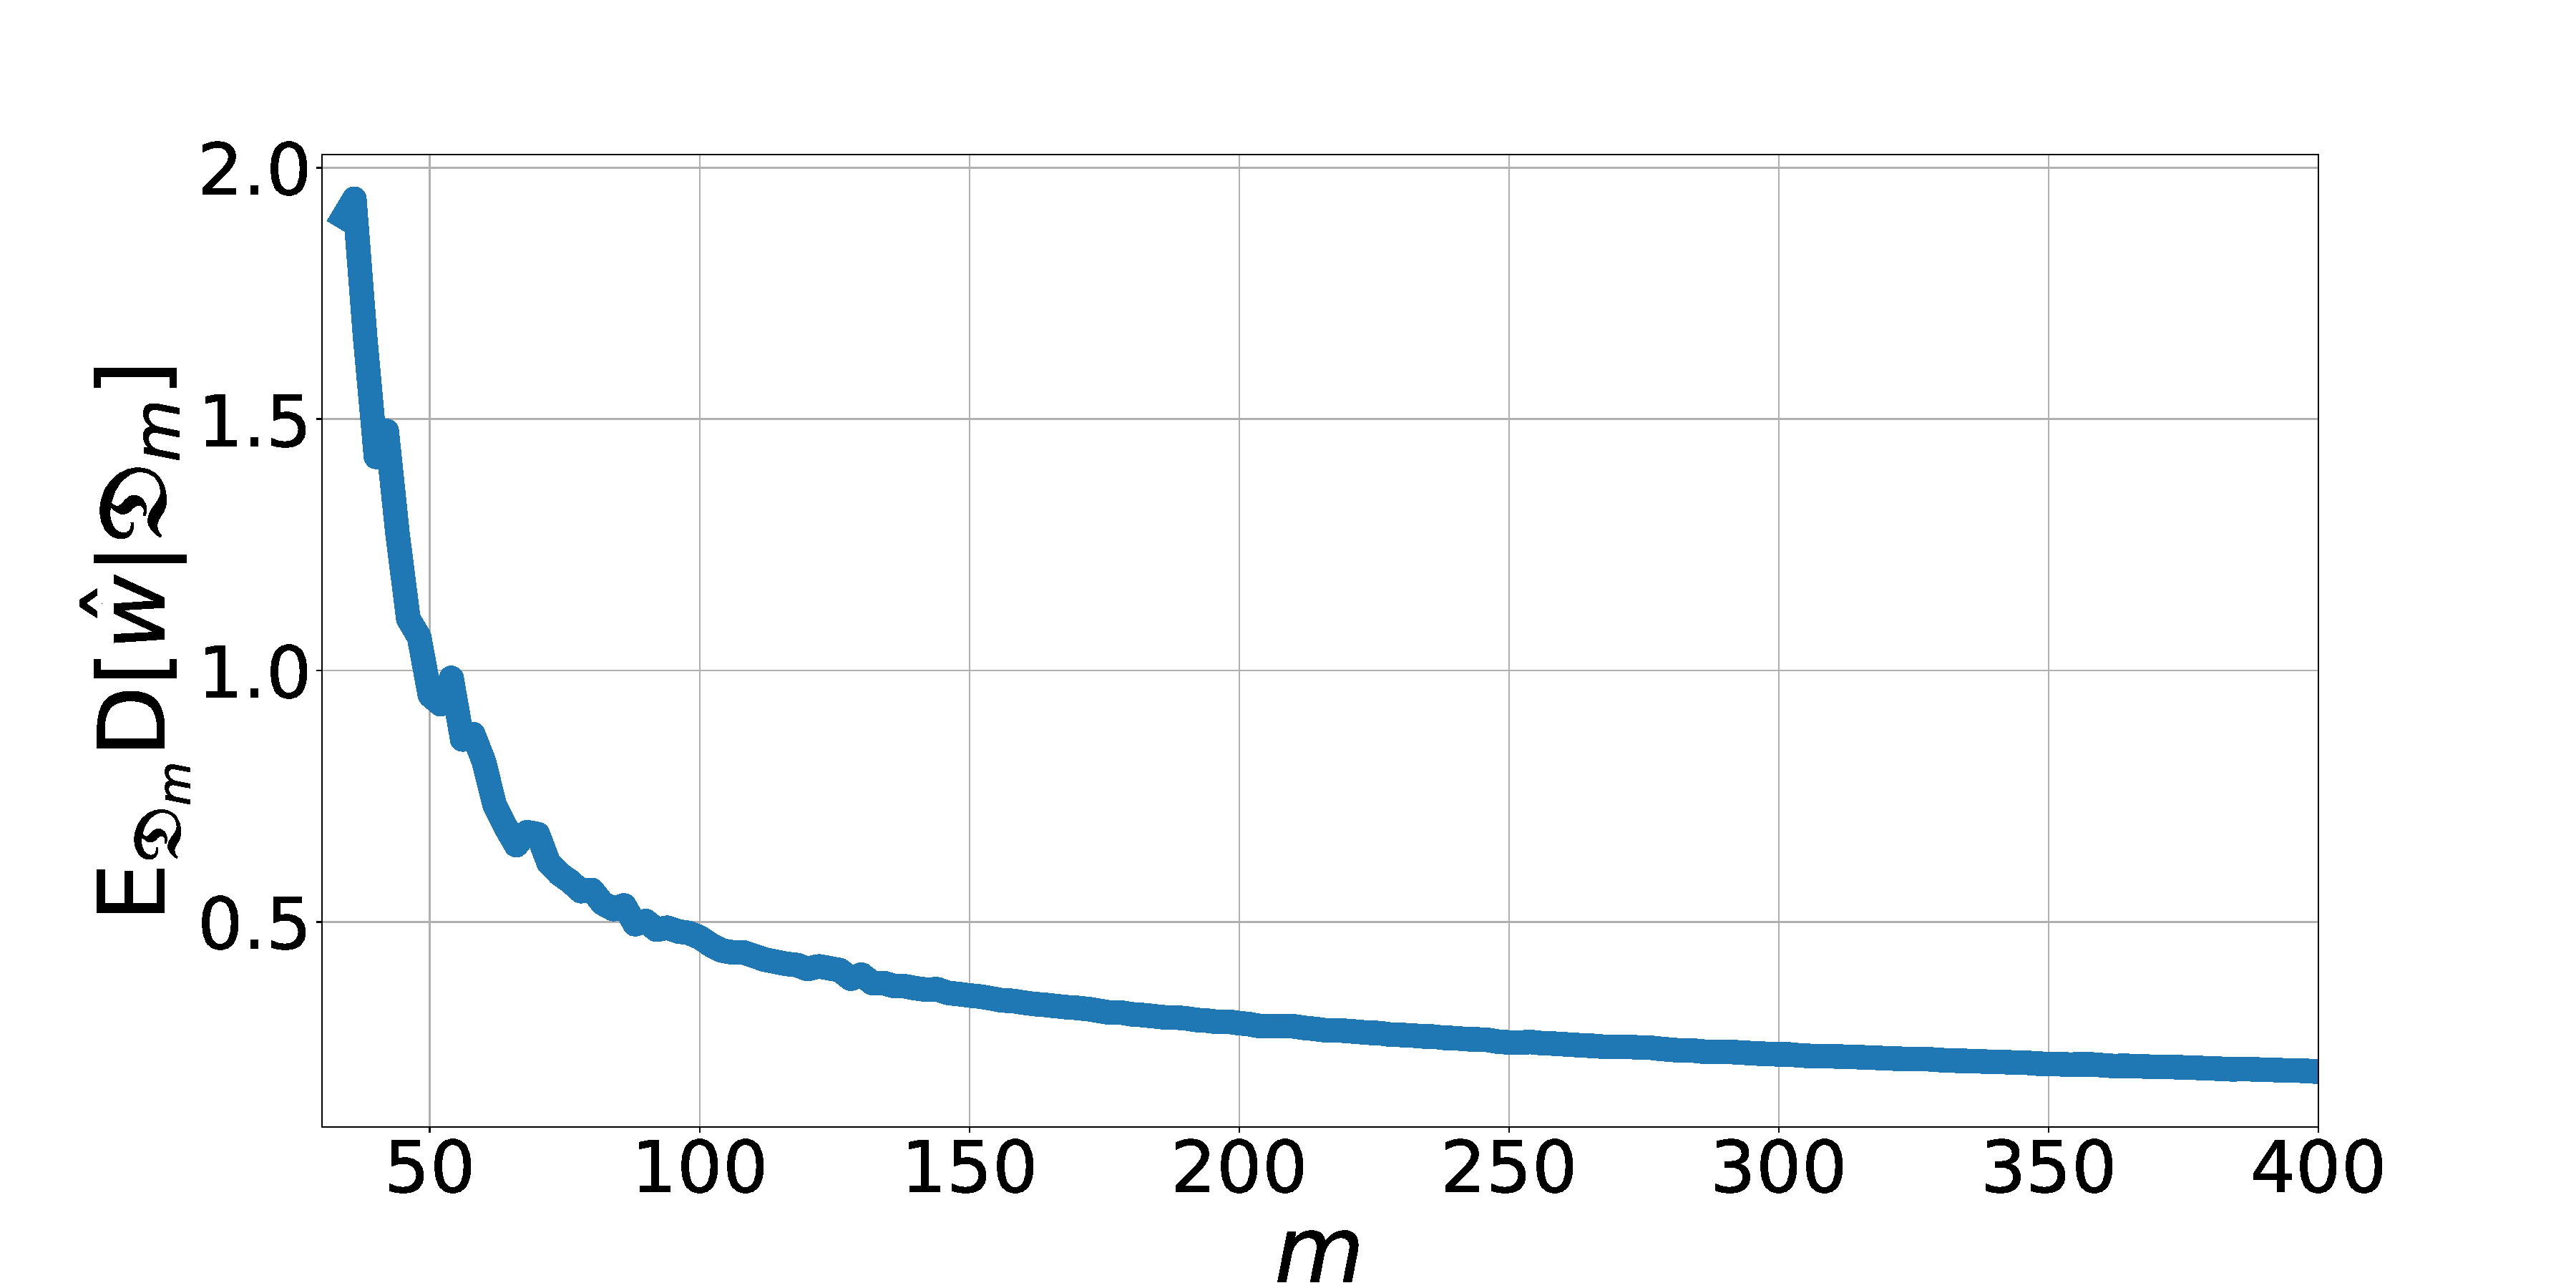
\includegraphics[width=0.49\textwidth]{results/samplesize/apvc.pdf}\\
    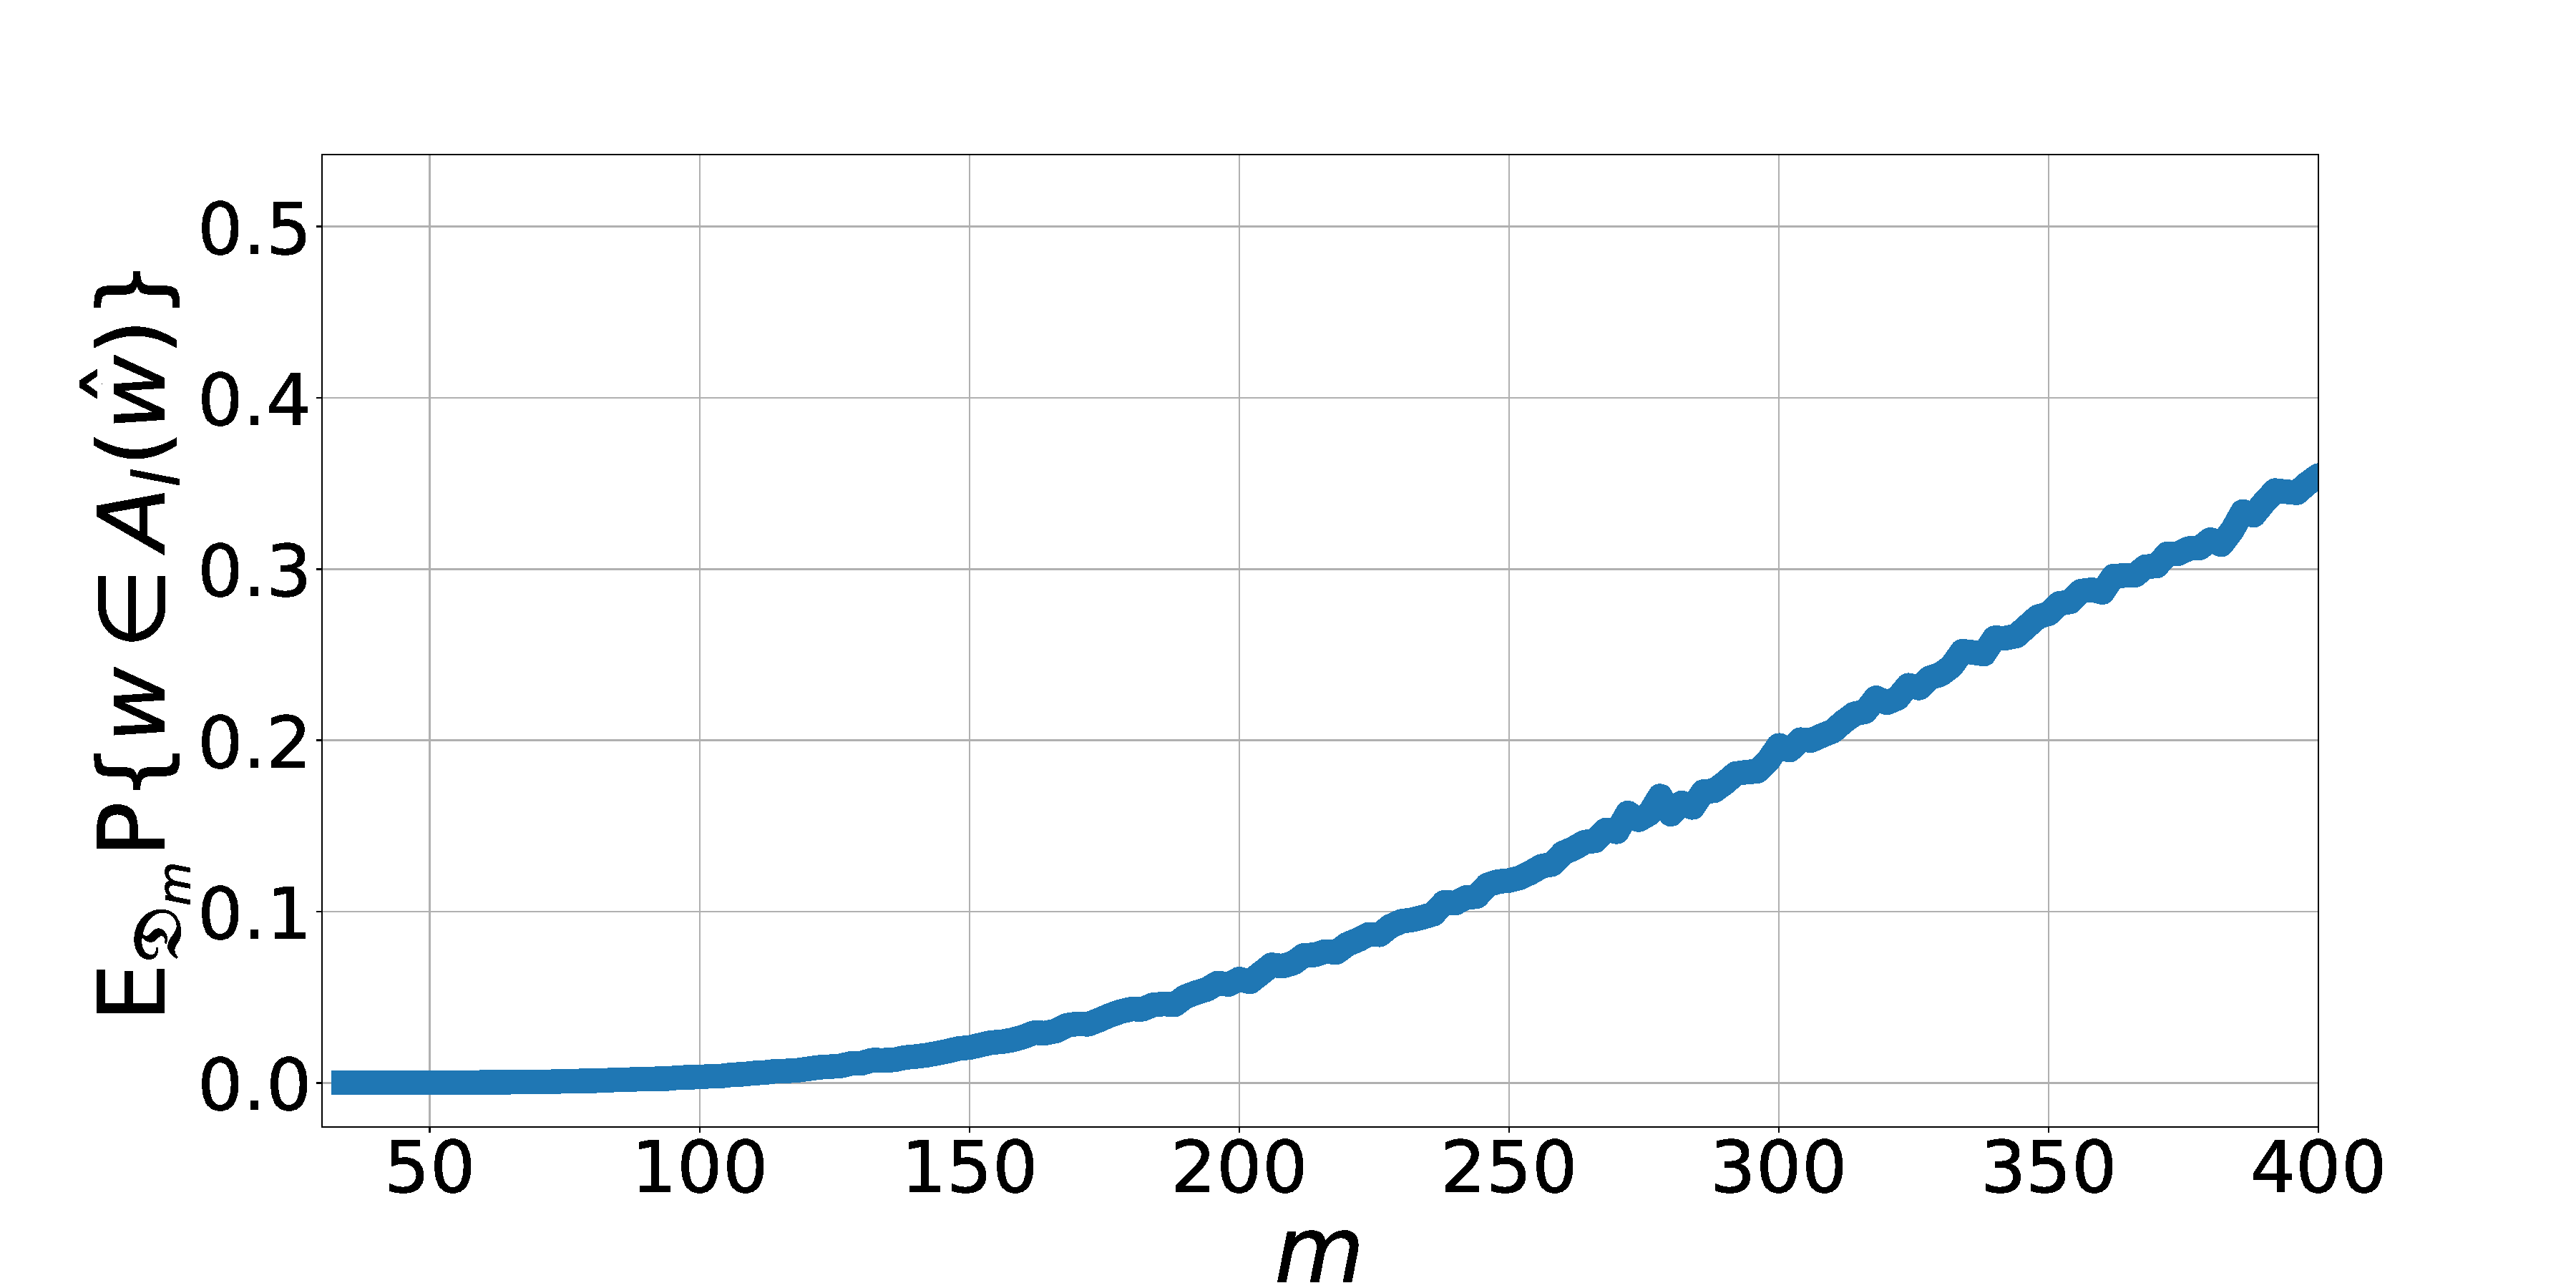
\includegraphics[width=0.49\textwidth]{results/samplesize/acc.pdf}
    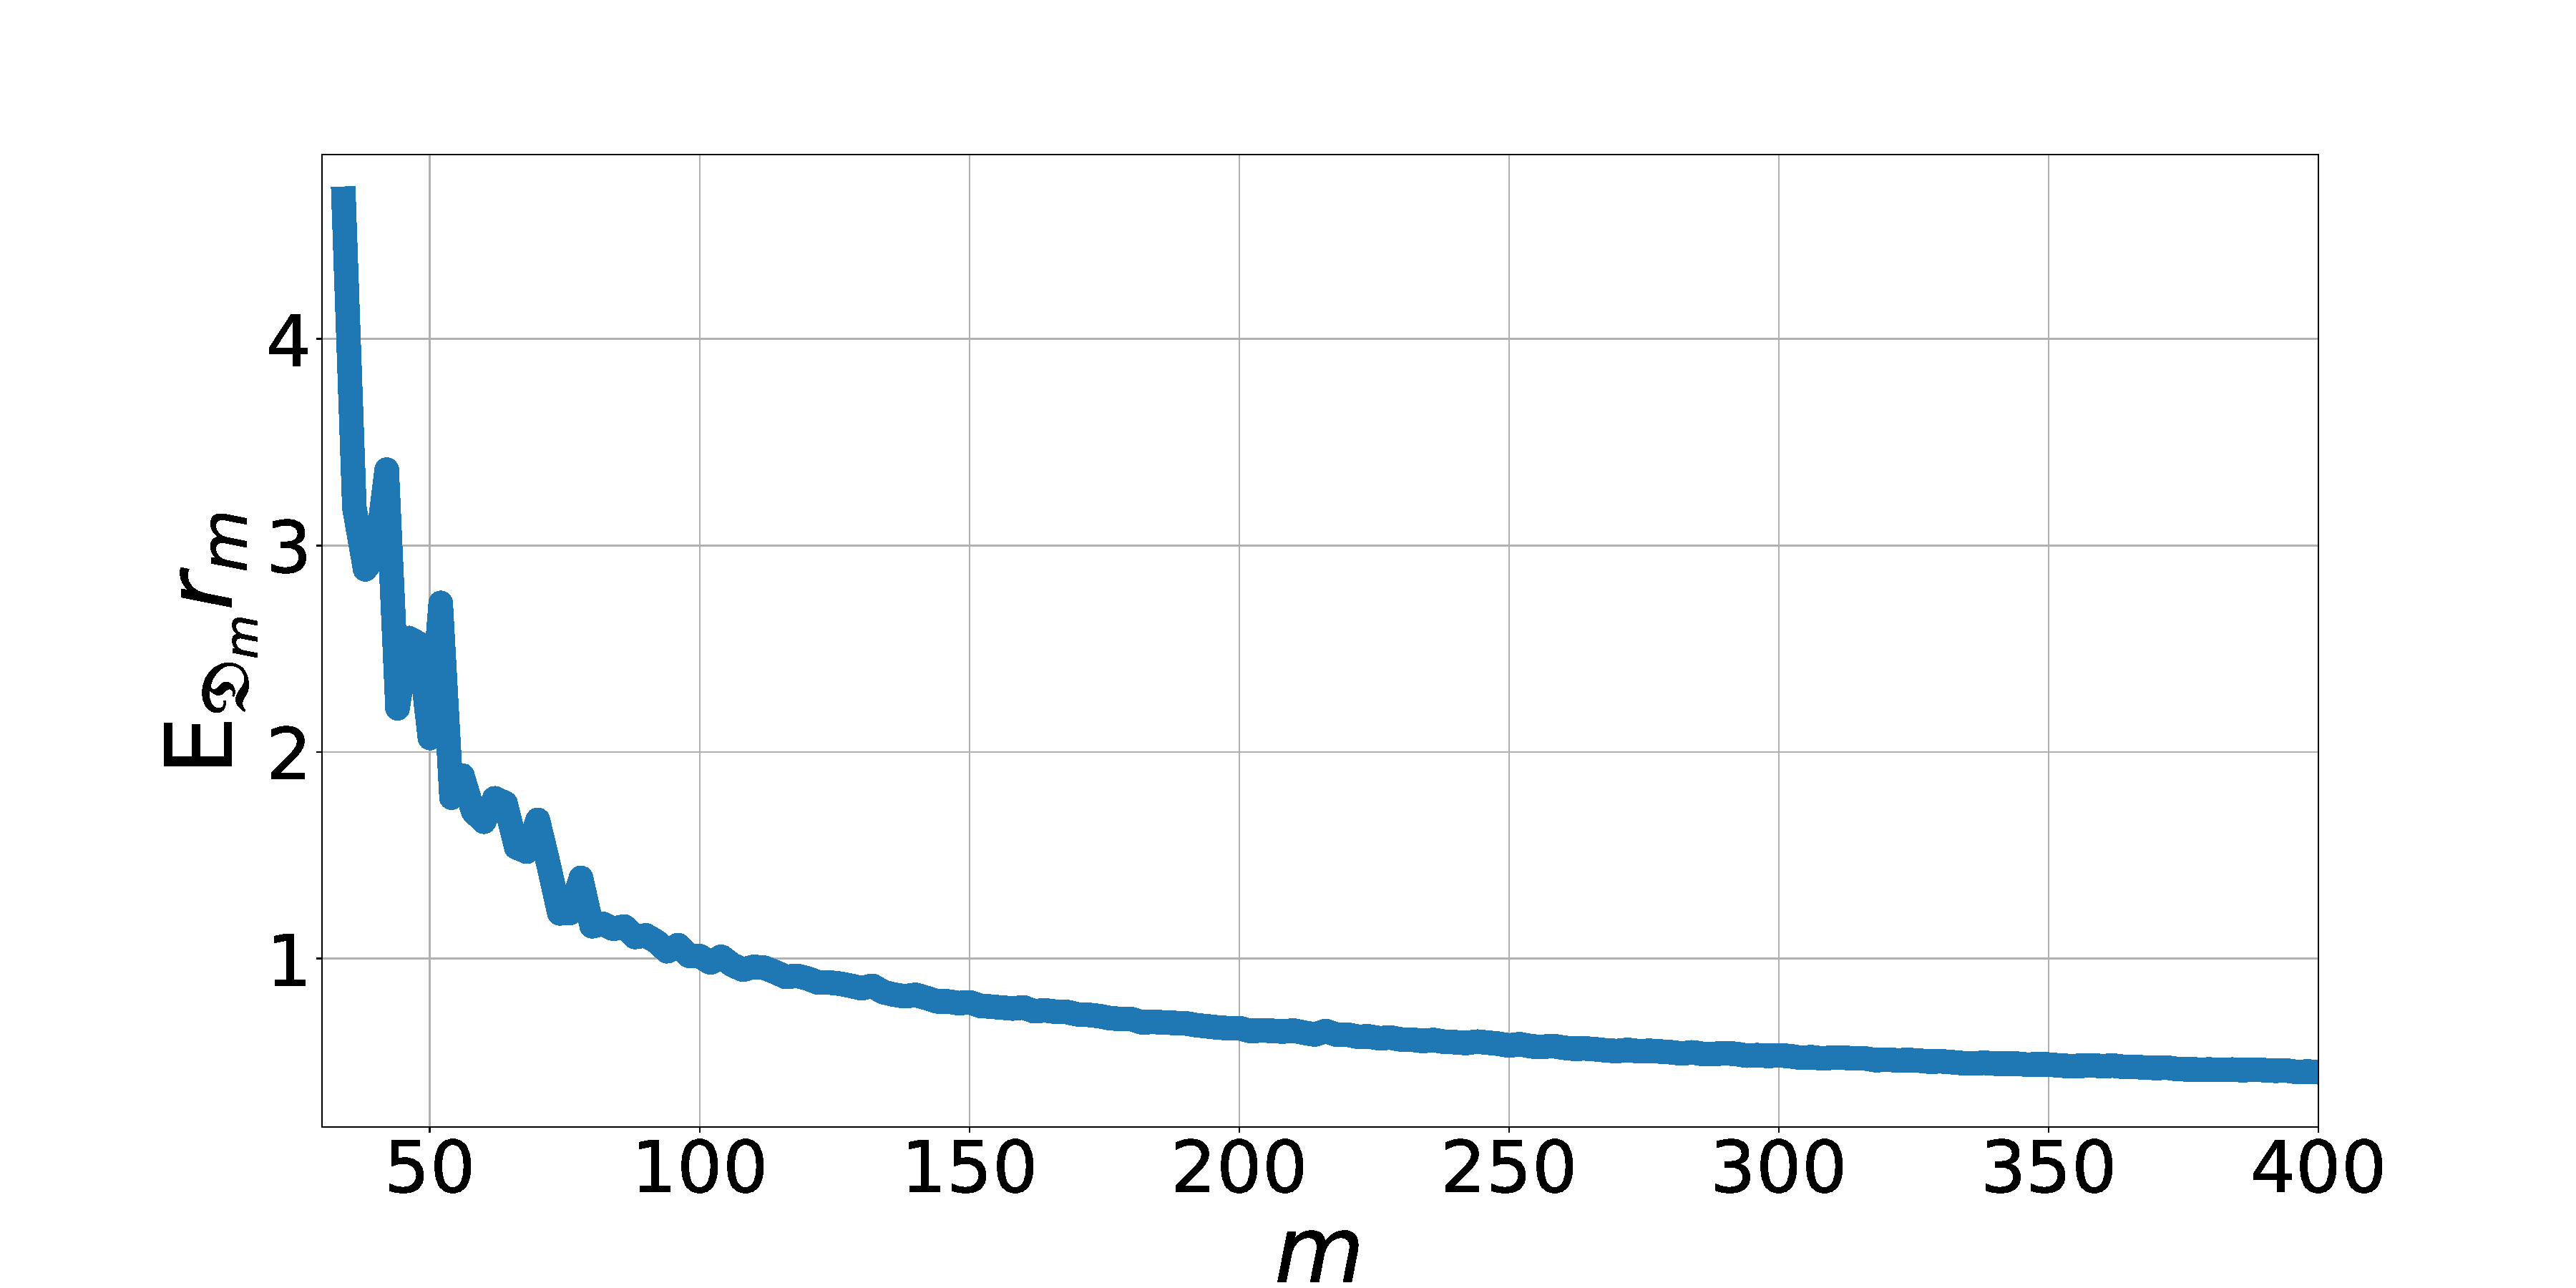
\includegraphics[width=0.49\textwidth]{results/samplesize/alc.pdf}\\
    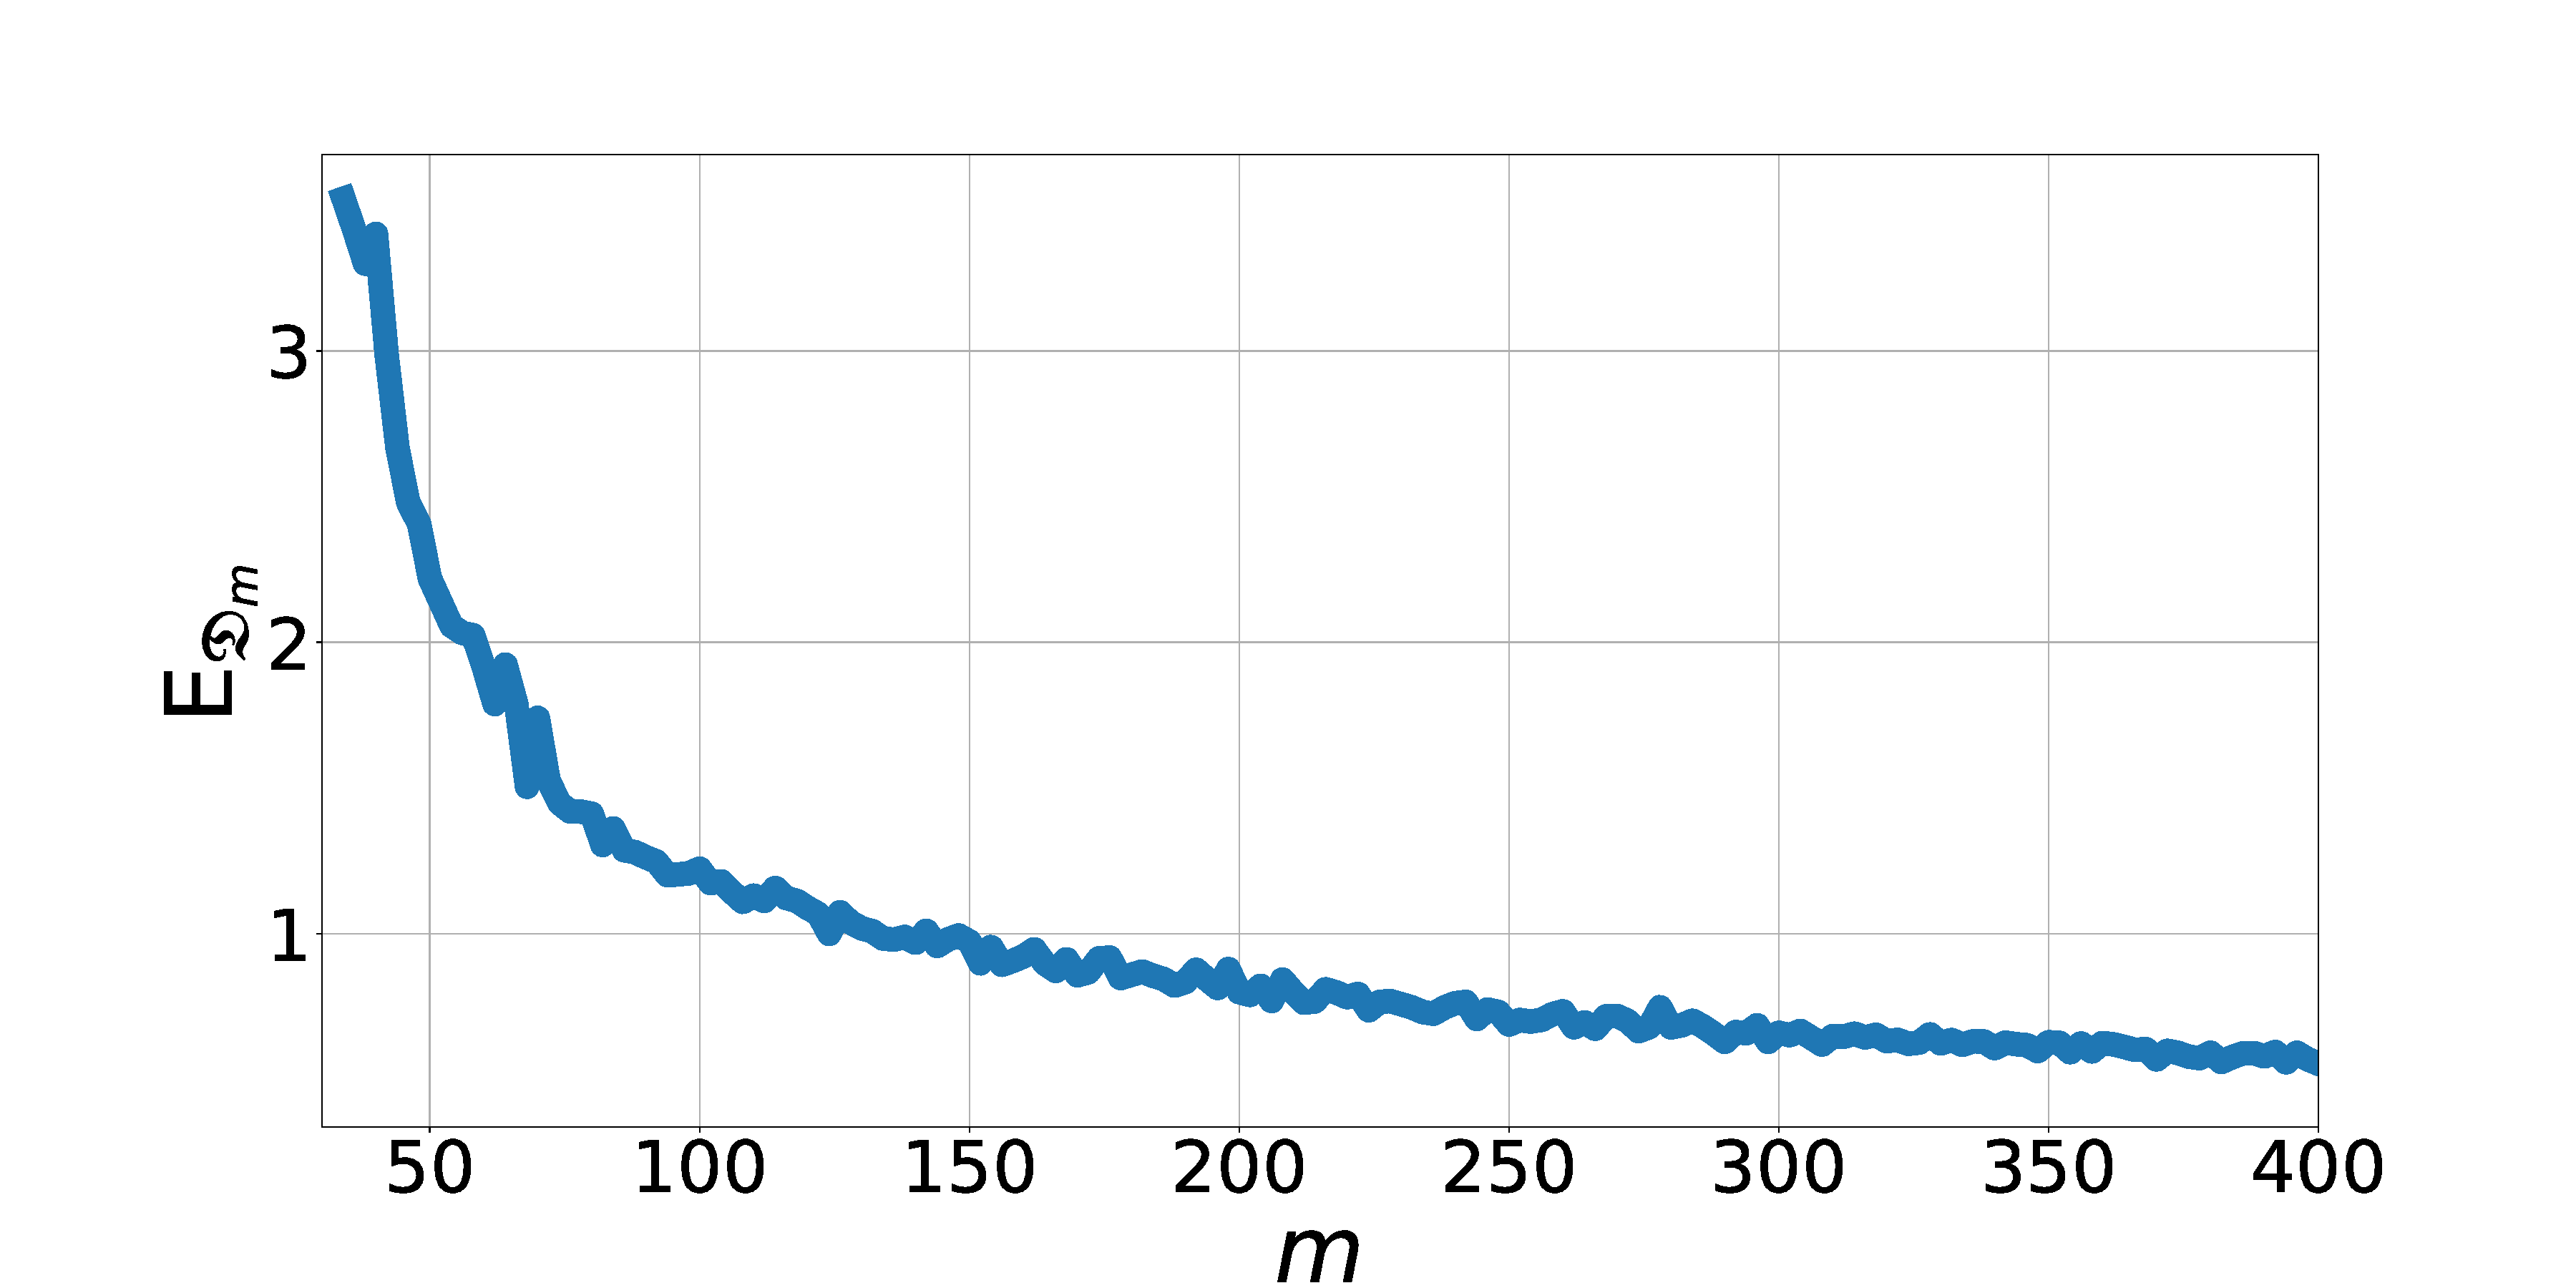
\includegraphics[width=0.49\textwidth]{results/samplesize/bootstrap.pdf}
    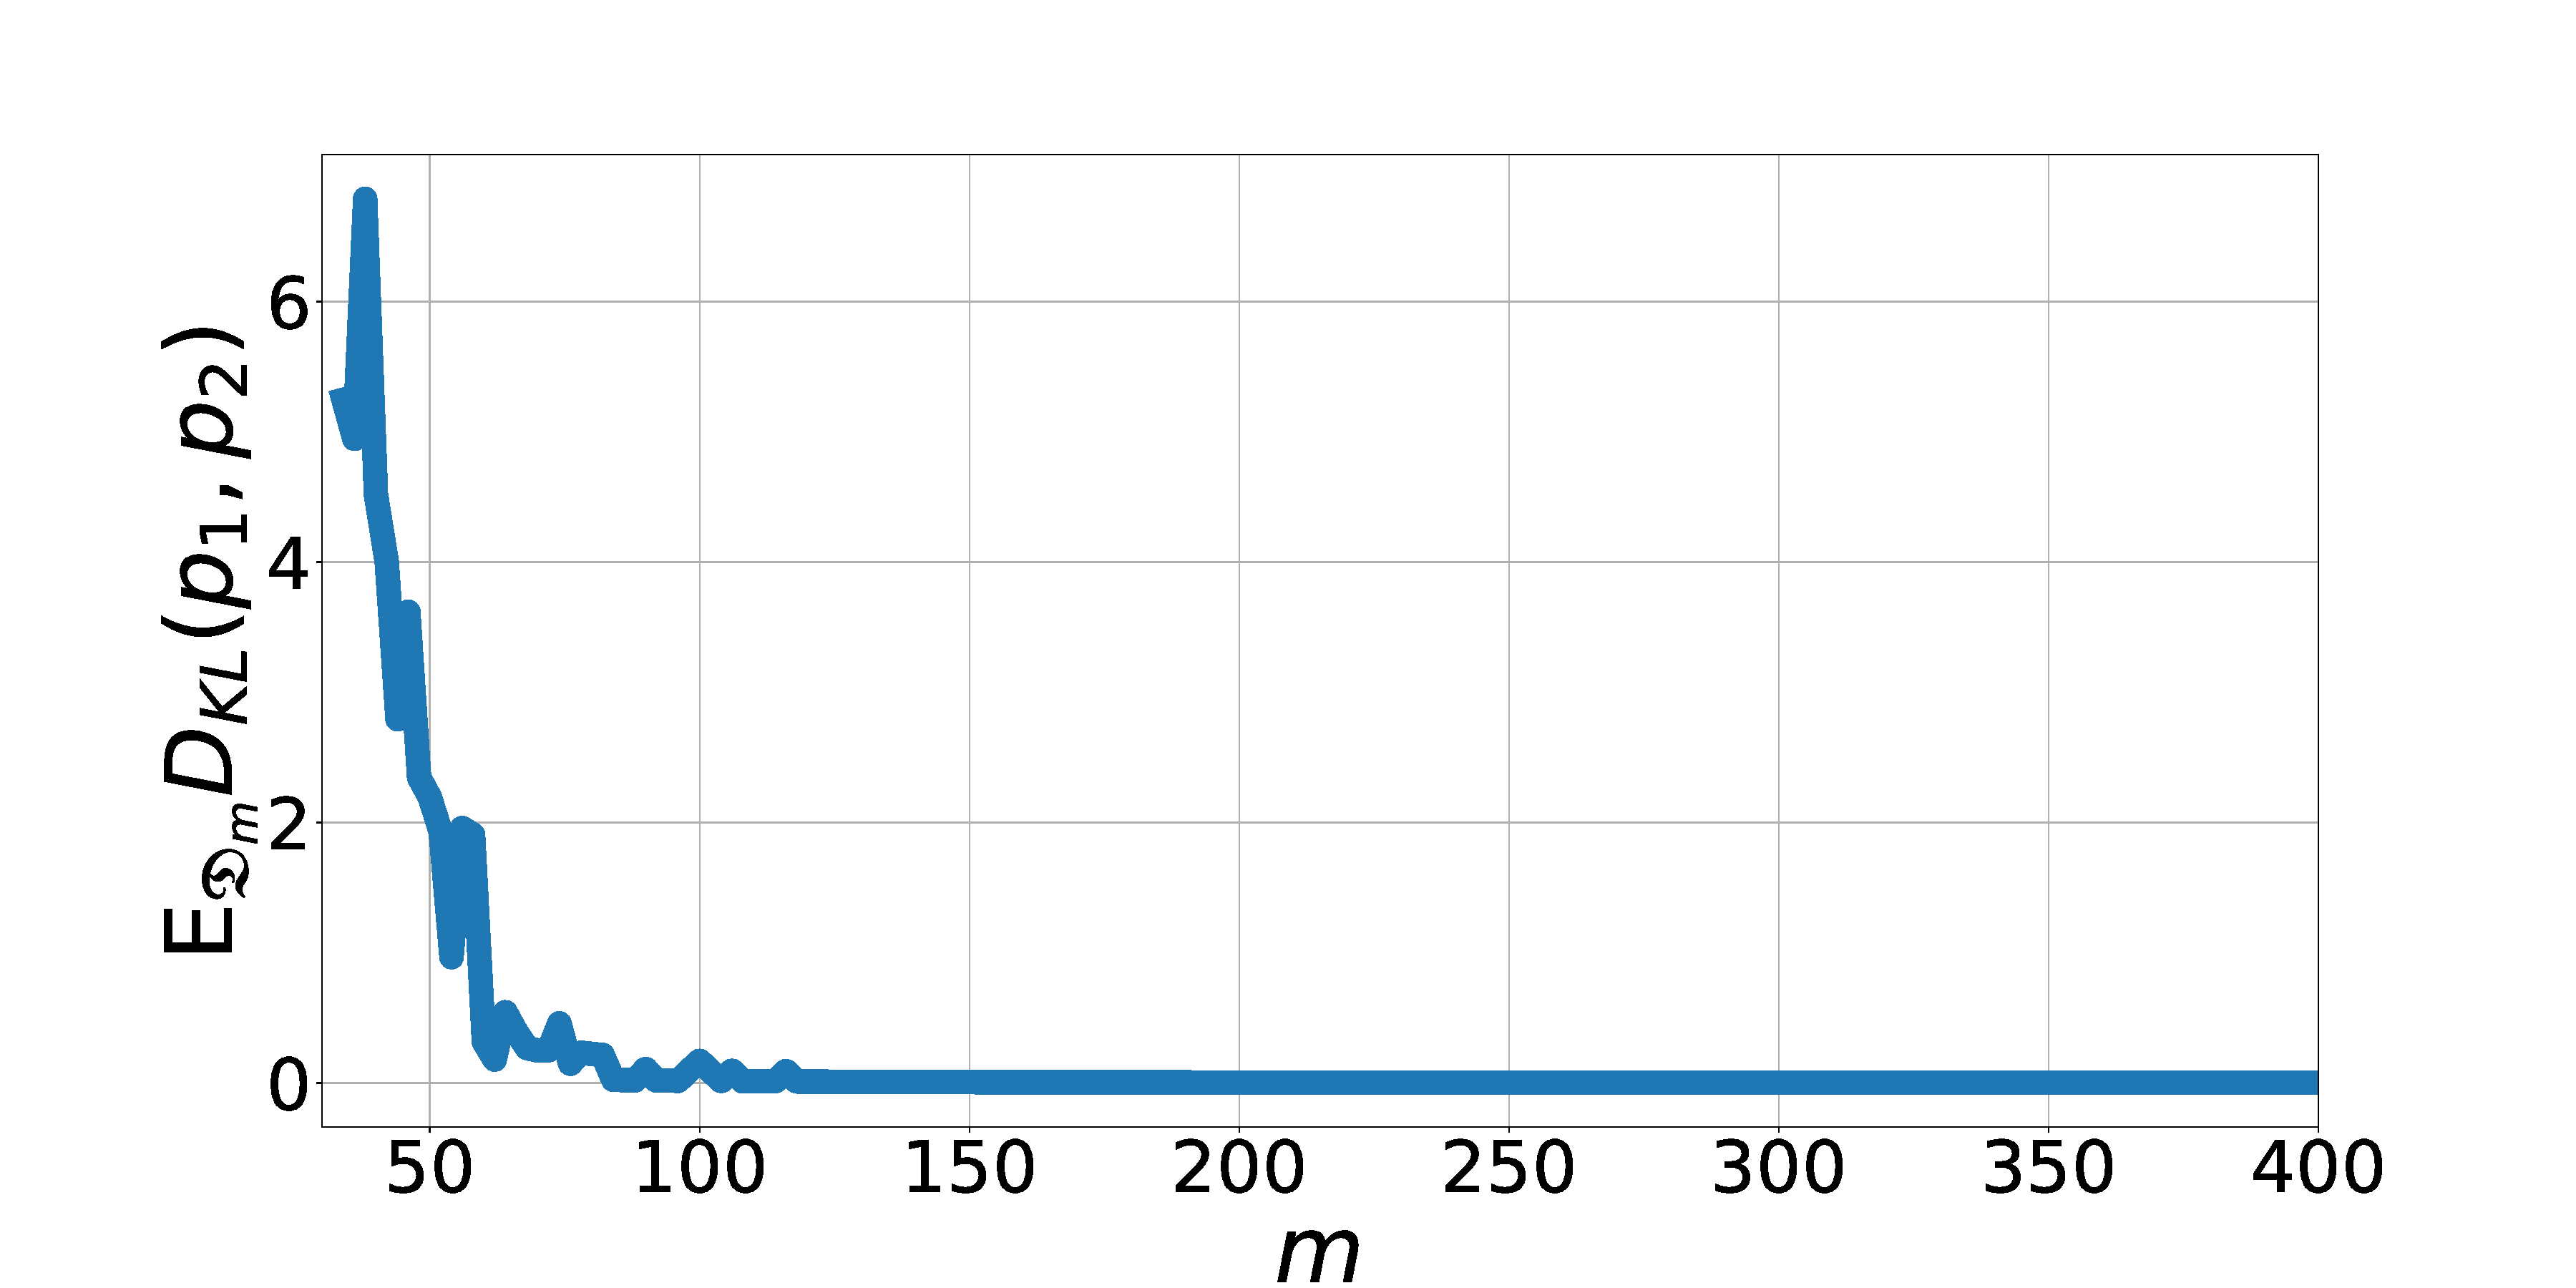
\includegraphics[width=0.49\textwidth]{results/samplesize/kl.pdf}\\
    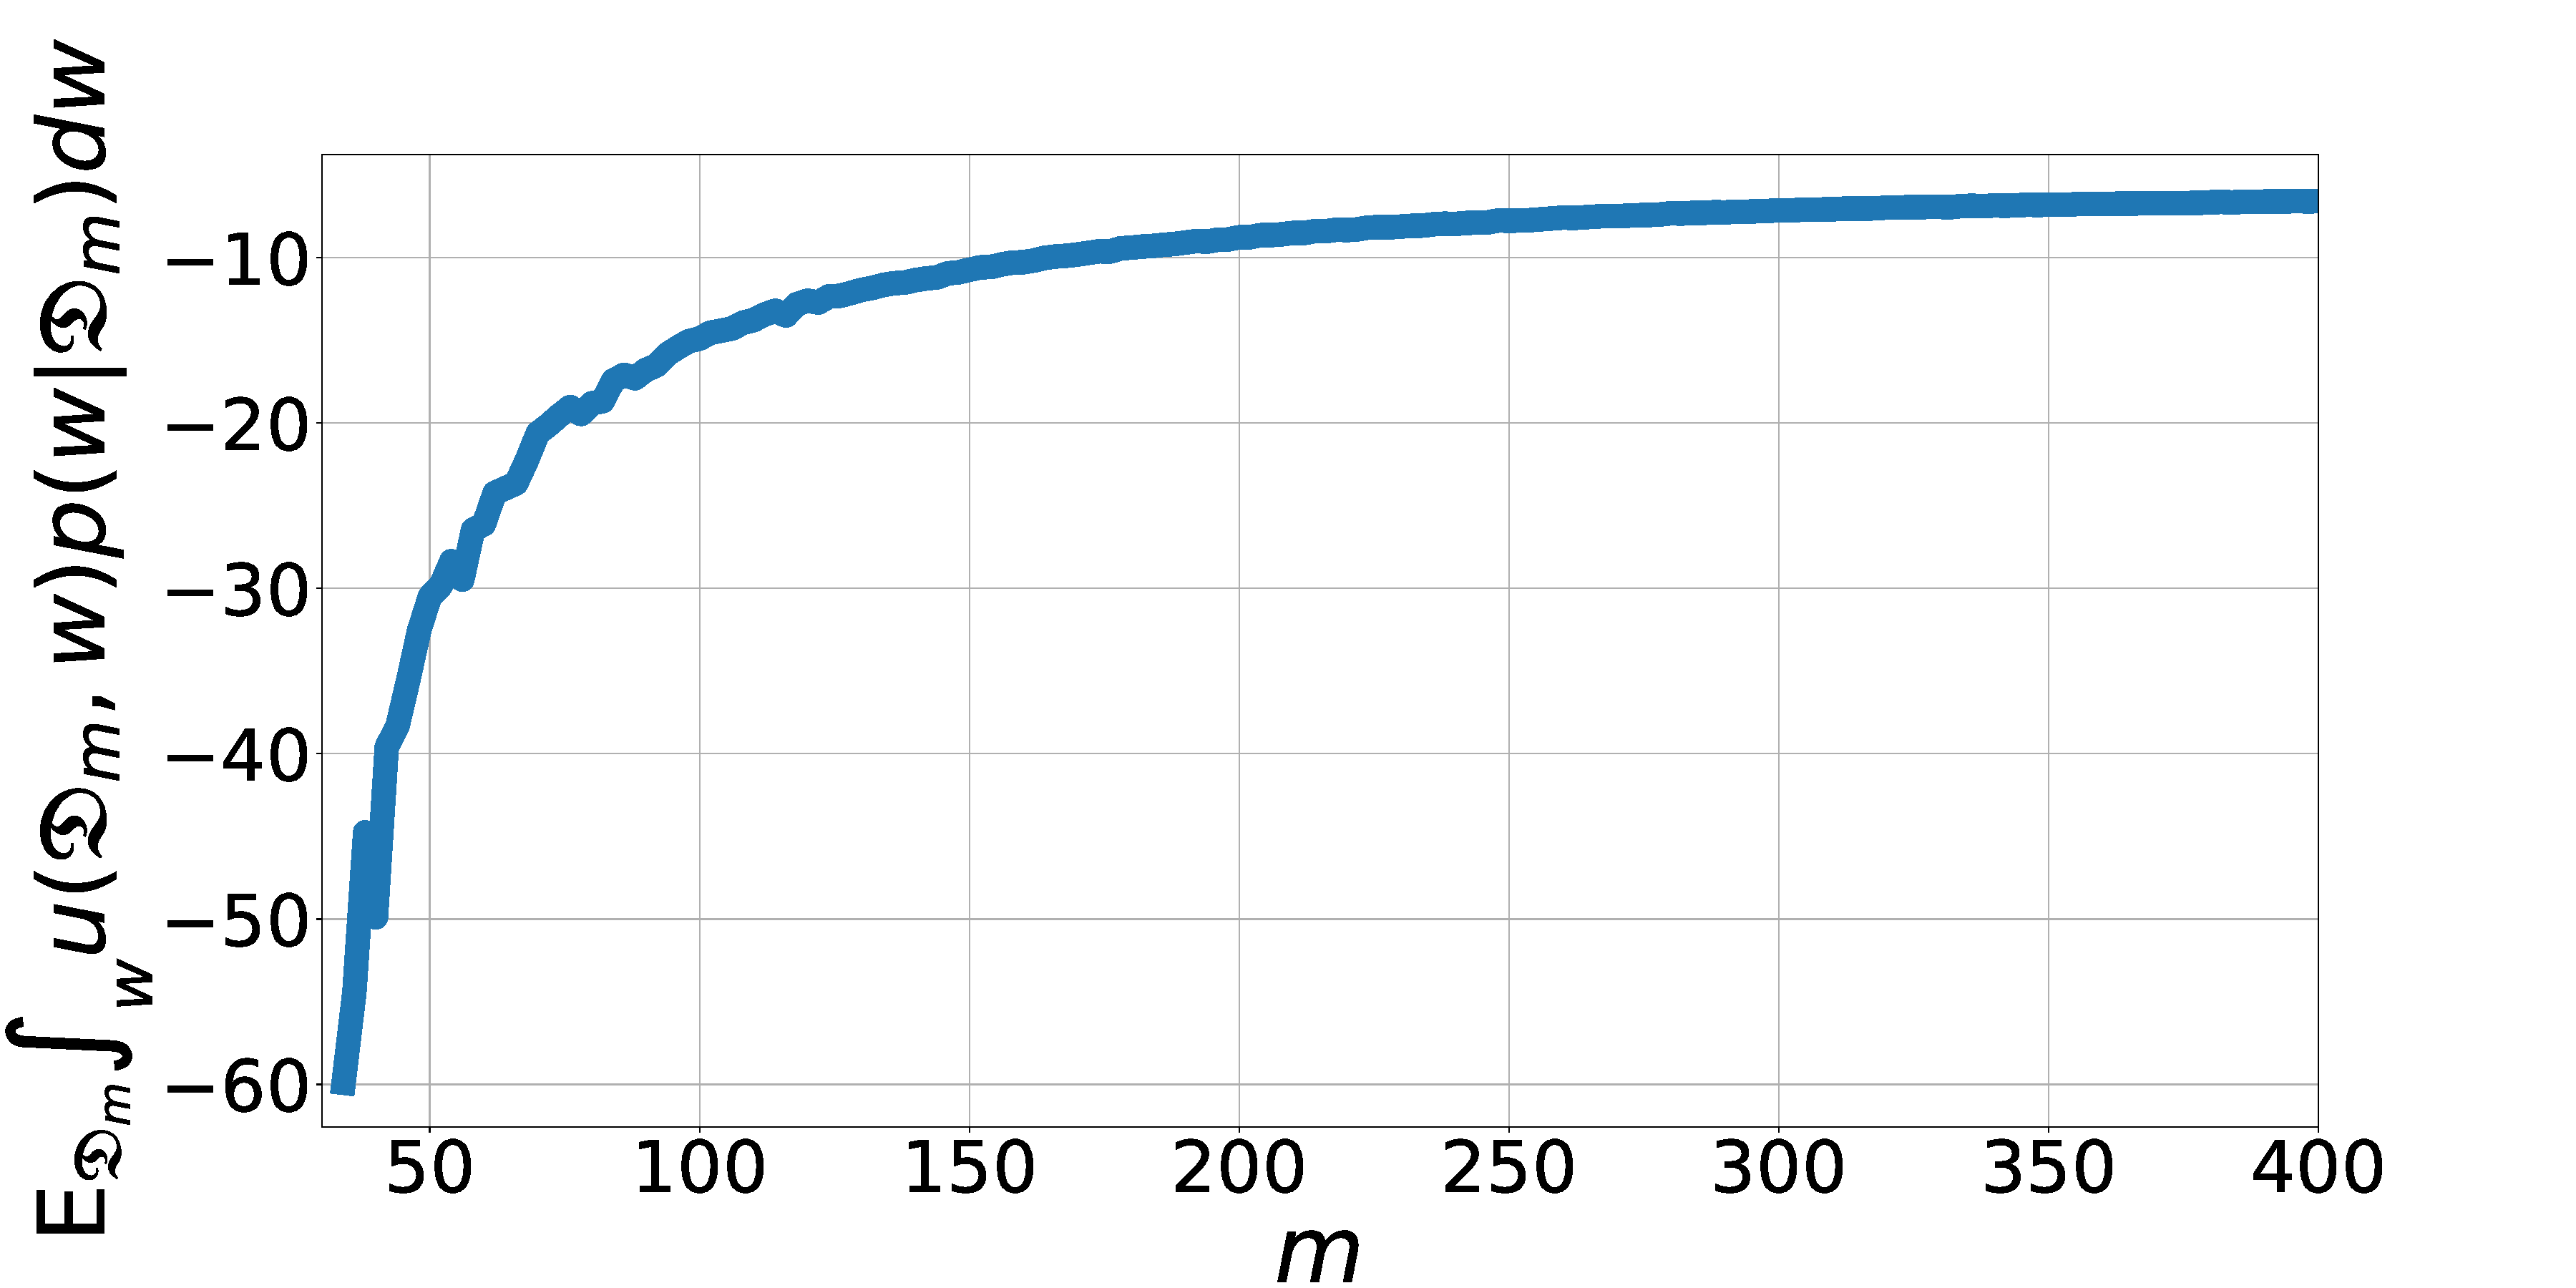
\includegraphics[width=0.49\textwidth]{results/samplesize/maxu.pdf}
    \caption{Поведение основных скалярных функций методов в зависимости от доступного объема выборки}
    \label{fig1}
\end{figure}

\begin{figure}[h!t]\center
    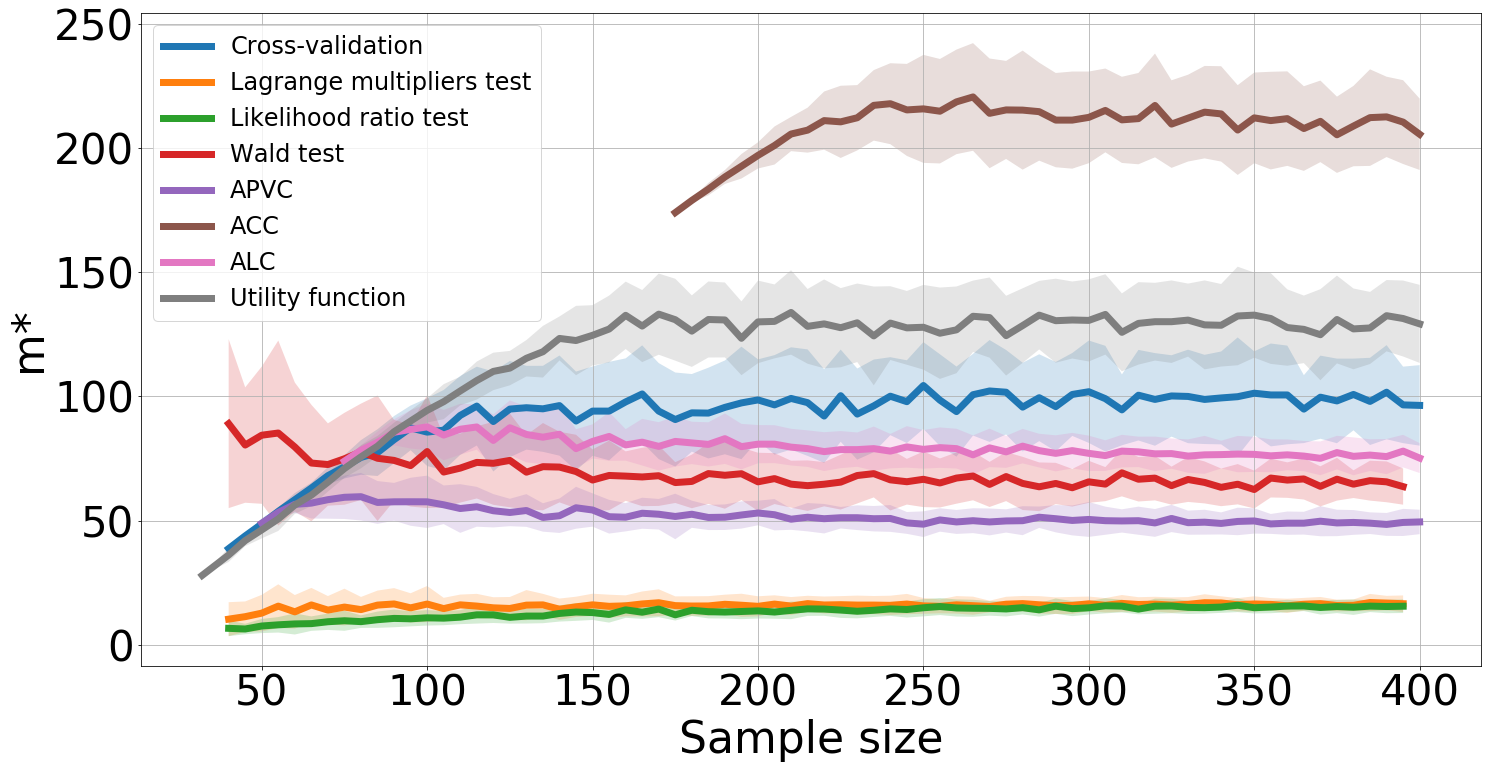
\includegraphics[width=0.85\textwidth]{results/samplesize/graphs.png}
    \caption{Поведение методов в зависимости от доступного размера выборки}
    \label{fig2}
\end{figure}

На рисунке \ref{fig1} показана зависимость статических значений каждого метода для каждого набора данных с фиксированным размером выборки $m$. Пороговые значения для каждого метода устанавливаются экспертно, что позволяет контролировать различные функции набора данных. Рисунок \ref{fig1} демонстрирует адекватность различных определений достаточности размера выборки. Все представленные функции монотонны и все они асимптотически стремятся к константе.
На рисунке \ref{fig2} показаны результаты методов на выборках разного размера. Он показывает, как методы различаются по дисперсии вычисленного $m^*$ и поведению в случае небольшого набора выборок. Методы сходятся, и результат становится независимым от  доступного размера выборки $m$.   
 

Малое значение дисперсия интерпретируется как вычислительная стабильность рассмотренных методов. Некоторые методы не могут дать оценку достаточного размера выборки, если у них нет соответствующего размера выборки. Это означает, что они не эфективны с точки зрения прогноза, но могут быть использованы для ретроспективы и анализа уже проведенного эксперимента.

В эксперименте также рассмотрена зависимость между оценкой размера выборки с помощью рассмотреных методов и доступного объема данных. Константа, достигаемая диаграммой зависимости $m^*$ от $m$, является прогнозом метода оптимального размера выборки. Если эта константа меньше $m$ там, где это показано на диаграмме, то метод прогнозирует оптимальный размер выборки до его получения. Таким свойством обладают только методы Лагранжа, Вальда и метод отношения правдоподобия.

Исследуется изменение оценки размера выборки в зависимости от изменения определенных гиперпараметров для байесовских методов, а также методов, основанных на перекрестной проверке и бутстрапе. Чтобы проанализировать поведение методов, рассмотрена выборка {Boston Housing}, остальные выборки имеют такую же тенденцию.
Байесовские методы, а также методы, основанные на перекрестной проверке и начальной загрузке, работают на основе определенного решающего правила для определенной выборочной функции. На рисунке \ref{fig1} показана зависимость этих функций от размера подвыборки. Как показано на рисунке \ref{fig1}, эти функции монотонно убывают или увеличиваются. Тип поведения функции зависит от метода. Изменяя ограничения, установленные экспертно, можно изменить размер выборки, который будет соответствовать этим ограничениям.
